
\chapter{Geodynamical/geophysical benchmarks \label{sec:geobench}}

\begin{flushright} {\tiny {\color{gray} \tt chapter\_benchmarks.tex}} \end{flushright}

%=======================================
\section{Benchmarks organised by topics}

Some published numerical experiments have over time become benchmarks for the entire
community. I present in what follows a short list of `famousx' benchmarks' in the 
computational geodynamics community.

%-----------------------------------
\subsection{Subduction}

\begin{itemize}
\item subduction problems: \textcite{spka06} (2006), \textcite{scbe08} (2008), 
                           \textcite{vack08} (2008), \textcite{cehg14} (2014),
                           \textcite{gltf18} (2018), \textcite{ozrs08} (2008),
                           \textcite{siwi20} (2020).

\item Benchmark of 3D numerical models of subduction against a laboratory experiment: 
      Meriaux \etal (2018)  \cite{memm18}

\end{itemize}

%-----------------------------------
\subsection{Stokes sphere \& sinkers}

\begin{itemize}
\item the Stokes sphere: Gale manual \cite{galemanual}, 
      \aspect{} manual \cite{aspectmanual}, 
      in visco-plastic fluid: \textcite{limd02} (2002), 
      \textcite{demj04} (2004). 
      Finite deformation in and around a fluid sphere \cite{sccm88,crud88}.

\item the sinking block (sinker) 
      \textcite{thie11} (2011),
      \textcite{cehg14} (2014),
      \textcite{gery10} (2010),
      \textcite{geyu03} (2003),
      \textcite{mamo08} (2008),
      \textcite{mishin11} (2011),
      \textcite{fumt11} (2011),
      \textcite{maie12} (2012),
      \textcite{sctc20} (2020),
      \textcite{mivg22} (2022). 
      (see Section~\ref{sec:sinker})

\item multiple sinkers \cite{mabl14,mabl15,clhe21,rusg17}

\item Sinking cylinder (2D Stokes sphere): 
      appendix A of \cite{boht08a}, \cite{wali04}.

\item hot blob problem \cite{bugs09,fumt11} (see Section~\ref{sec:hotblob})
\end{itemize}


%-----------------------------------
\subsection{(Visco-)Elastic deformation}

\begin{itemize}

\item bending of elastic plate/beam \cite{cehg14,boht08a,vosc15,elga10,demh19,modm02,litu02}

\item flexure of finite length elastic plate \cite{chtl13}

\item stress build-up in Maxwell visco-elastic material 
      \cite{geyu07,chtl13,elga10,demh19}
\item single layer visco-elastic folding \cite{scps01,vosc15}
\item viscous(-elastic) flow around a cylinder in a channel (see Section~\ref{sec:flowcyl})
\item Semi-infinite elastic half plane with a circular hole \cite{verr98}
\item Uniform strip load on elastic material (see Section~\ref{sec:elaststripload})
\item Jull and McKenzie (1996) \cite{jumc96} parabolic load on viscoelastic half-space (and melt fractions) 
\item Stress distribution in elastic sphere under equal and 
      opposite loads \cite{stro52}
\item Love's problem: Becker \& Bevis (2004) \cite{bebe04}
\item Infinite plate with a circular hole \cite{yiha10,rama16}
\item Square plate with a crack subjected to a horizontal tensile 
      traction \cite{litu02}
\item Hollow sphere under internal pressure, see Section~\ref{ss:hollowsphereintpress}
\end{itemize}

%-----------------------------------
\subsection{Convection}

\begin{itemize}
\item 2D Rayleigh-Benard convection (see Section~\ref{ss:blbc89}).

\item 2D Rayleigh-Benard convection, lateral heating, 30+ codes: 
      \textcite{dejo83} (1983).

\item 2D Rayleigh-Benard convection with nonlinear rheology:  
      \textcite{tosn15} (2015), \aspect{} manual \cite{aspectmanual}, 
      \textcite{trbs21} (2021), \stone~28, \textcite{dakg22} (2022),
      \textcite{siwi20} (2020), \textcite{casd20} (2020).

\item 3D convection at infinite Prandtl number with modest viscosity variation:
      \textcite{bucc94} (1994),
      \textcite{trha98} (1998),
      \textcite{kaks05} (2005),
      \textcite{onmm06} (2006),
      \textcite{krhb12} (2012), 
      \textcite{trbs21} (2021),
      \textcite{dakg22} (2022).
      This benchmark is carried out in Stone~\ref{f20}.

      \begin{center}
      \includegraphics[height=4cm]{images/busse93/kaks05}
      \includegraphics[height=4cm]{images/busse93/krhb12}\\
      {\captionfont Left: Taken from Kameyama \etal (2005).
      a) Isothermal surfaces obtained for the benchmark calculations 
      of stationary convections in Busse \etal. (1993). (a) Case 1a is for
      constant viscosity, while (b) Case 2 is for modestly temperature-dependent 
      viscosity whose viscosity contrast is 20. The calculations
      were carried out with (a) 64x32x64 and (b) 64x64x64 mesh divisions.
      Right: Taken from Kronbichler \etal (2012).}
      \end{center}

\item Numerical simulations of three-dimensional thermal convection 
      in a fluid with strongly
      temperature-dependent viscosity: Ogawa \etal \cite{ogsz91,kaks05} 

\item Convection in 2D-box \cite{galb19} (see Section~\ref{sec:citb})

\item Onset of convection \cite{aspectmanual}

\item mantle convection in 3D spherical shell:
      \textcite{rasz96} (1996),
      \textcite{iwas96} (1996),
      \textcite{zhzm00} (2000),
      \textcite{yoka04} (2004),
      \textcite{sthh06} (2006),
      \textcite{chcc07} (2007),
      \textcite{zhmt08} (2008),
      \textcite{kaks08} (2008),
      \textcite{wrfy10} (2010),
      \textcite{dadb13} (2013),
      \textcite{busa13} (2013),
      \textcite{arfw14} (2014),
      \textcite{liki19} (2019),
      \textcite{trbs21} (2021),
      \textcite{eulg23} (2023),
      \textcite{ildk24} (ildk24).

\item Mantle convection with reversing mobile plates \cite{kogk05}

\item A comparison of mantle convection models featuring plates \cite{stlh14}

\end{itemize}

%-----------------------------------
\subsection{Free surface \& interfaces}

\begin{itemize}

\item Free surface evolution: Crameri \etal (2012) \cite{crsg12}, 
      \aspect{} manual \cite{aspectmanual}, \textcite{sctc20} (2020).

\item relaxation of sinusoidal interface \cite{crsg12,robh17}

\end{itemize}


%-----------------------------------
\subsection{Rayleigh-Taylor}

\begin{itemize}
\item 2D Rayleigh-Taylor convection/instability:\\ 
      \textcite{pros81} (1981),
      \textcite{trab90} (1990),
      \textcite{wesc92} (1992),
      \textcite{popo92} (1992),
      \textcite{ogaw93} (1993),
      \textcite{como97} (1997),
      \textcite{vaks97} (1997),
      \textcite{devv00a} (2000),
      \textcite{soga01} (2001),
      \textcite{bast02} (2002),
      \textcite{taki03} (2003),
      \textcite{bomh06} (2006),
      \textcite{dadh07} (2007),
      \textcite{basd08} (2008),
      \textcite{deka08} (2008),
      \textcite{qurj09} (2009),
      \textcite{saev10} (2010),
      \textcite{sunh10} (2010),
      \textcite{lezh11} (2011),
      \textcite{thie11} (2011),
      \textcite{mishin11} (2011), 
      \textcite{lomw12} (2012), 
      \textcite{maie12} (2012),
      \textcite{fusc13} (2013), 
      \textcite{vyrc13} (2013), 
      \textcite{chtl13} (2013),
      \textcite{ropu19} (2019),
      \textcite{robe19} (2019), 
      \textcite{demh19} (2019),
      \textcite{logb20} (2020),
      \textcite{sctc20} (2020),
      \textcite{mivg22} (2022),
      \textcite{buoa24} (2024),
      \aspect manual \cite{aspectmanual}.

\item 3D Rayleigh-Taylor instability:
      \textcite{fukk08} (2008),
      \textcite{vosc15} (2015).

\item Polydiapirism \cite{wesc92,aspectmanual}

\end{itemize}

%-----------------------------------
\subsection{Couette \& Poiseuille flow}

\begin{itemize}
\item Couette flow with temperature dependent viscosity \cite{elga10,demh19}
\item Couette flow with shear heating \cite{elga10}
\item Couette flow of a power-law fluid, Section 2.4 of  \textcite{saramito}
\item Poiseuille flow: \cite{fojg94,fuku11,tagm09} (see Section~\ref{ss:poiseuille})
\item Poiseuille-Couette flow: \textcite{fusc13} (2013)
\item Poiseuille flow of a power-law fluid, Section 2.3 of  \textcite{saramito}
\item Channel flow: \textcite{manc08} (2008)
\item channel flow (nonlinear): \cite{geyu03,maie12,frbt19,gery10,elga10}
\item Squeezing flow between moving parallel plates: \textcite{gugu77} (1977)
\item Flow of a Power Law Fluid Through a Tube - page 87 of \textcite{macosko}
\end{itemize}



%-----------------------------------
\subsection{Thermal problems}

\begin{itemize}
\item thermal diffusion of half-cooling space (see Section~\ref{sec:hcsp}) 
\item thermal diffusion of Gaussian distribution (see compgeo notes, elefant manual)
\item Heat flow around a cylinder (see Section~\ref{sec:hfcyl})
\end{itemize}

%-----------------------------------
\subsection{Lid driven cavity problems}

\begin{itemize}
\item Lid driven cavity 
      \textcite{kawa61} (1961),
      \textcite{chor67} (1967),
      \textcite{shry78} (1978),
      \textcite{foth79} (1979),
      \textcite{ghgs82} (1982),
      \textcite{kost84} (1984),
      \textcite{bope98} (1998),
      \textcite{xika01} (2001),
      \textcite{brsa06} (2006),
      \textcite{ertu09} (2009),
      \textcite{tesk12} (2012).

\item Lid driven cavity with analytical solution (see Section~\ref{sec:ldc_anal})

\item Lid driven cavity with nonlinear rheology \cite{been80,svna18}
\end{itemize}

%-----------------------------------
\subsection{Visco-plastic problems}

\begin{itemize}

\item the 'plastic brick' (See section~\ref{ss:plasticbrick}): \\
      \textcite{lemm08} (2008), 
      \textcite{qurj09} (2009), 
      \textcite{kaus10} (2010), 
      \textcite{mishin11} (2011), 
      \textcite{muso11} (2011), 
      \textcite{maie12} (2012), 
      \textcite{spmw16} (2016), 
      \textcite{kapb16} (2016), 
      \textcite{gltf18} (2018), 
      \textcite{frbt19} (2019),
      \textcite{mivg22} (2022).

\item indentor, punch problem (see Section~\ref{sec:punch}):\\
      \textcite{vidm82} (1982),
      \textcite{vidm84} (1984),
      \textcite{vimd86} (1986),
      \textcite{hukm03} (2003), 
      \textcite{fojd04} (2004), 
      \textcite{thfb08} (2008),
      \textcite{gerb12} (2012), 
      \textcite{gltf18} (2018).

\item numerical sandbox \cite{bube06,bube06,maie12,busa16,gltf18}

\item fractal networks of shear bands: \textcite{pohe94} (1994)

\end{itemize}


%-----------------------------------
\subsection{Miscellaneous}

\begin{itemize}

\item 2D Rayleigh-Benard laminar plumes, comparison of laboratory 
      and numerical modeling : 
      \textcite{vavl09} (2009
)
\item 2D Cartesian flow with extremely temperature-dependent viscosity:
      \textcite{moso95} (1995), \textcite{trbs21} (2021).

\item Thin layer entrainment (see Section~\ref{sec:tlentr})

\item 1D compression \cite{modm02}

\item 2D compressible Stokes flow problem \cite{itki94,tagu07,lezh08,kilv10,lizh13}

\item Wannier flow \cite{wann50,yemu99,cehg14}

\item plastic oedometer test  \cite{chtl13}

\item Three-dimensional folding of an embedded viscous layer in 
      pure shear \cite{flet91}

\item dam-break problem 
      \cite{moeb99,bacp07,liir07,lemx08,homa09,anco09,grdn97,hini81,basd08}

\item Slope stability for elasto-plastic materials \cite{rama16}

\item Time-dependent flow in an annulus \cite{galb19} (see Section \ref{sec:tdba})

\item Slab detachment benchmark (see Section~\ref{sec:slabdetach}) 

\item 3D Hollow sphere Stokes flow benchmark:\\
      Thieulot (2017) \cite{thie17},
      Horbach \etal (2020) \cite{homb20},
      Kramer \etal \cite{krdw21}

\item Axisymmetric hollow sphere compressible Stokes flow benchmark:\\
      Machetel \& yuen (1989) \cite{mayu89}

\item Annulus benchmark \cite{aspectmanual}, \cite{ples11}

\item Viscosity grooves benchmark \cite{aspectmanual}

\item Latent heat benchmark \cite{aspectmanual}

\item Layered flow with viscosity contrast \cite{aspectmanual} 
      (see Section \ref{sec:layfl}) 

\item Brittle thrust wedges benchmark \cite{busa16,aspectmanual}

\item Laplace equation on a semi infinite plate (see Section~\ref{sec:lapplate})

\item 2D Stokes flow over cavity: Popov \& Makeev (2014) \cite{poma14}.

\item Analytical solution for solitary porosity waves: \textcite{copo15} (2015)

\item Analytical solution for solitary wave of magma: Dannberg \& Heister (2016) \cite{dahe16} and refs therein

\item Stokes flow caused by the motion of a rigid sphere close 
      to a viscous interface: \textcite{dagr98} (1998)

\item Deformation caused by a closed vertical volcanic pipe \cite{boda99}

\item Linear Stability Analysis for Thermal Convections in 
      Spherical Shells \textcite{yuwa19} (2019)

\item Viscous half-space loading \cite{hask35}

\item Nakiboglu and Lambeck (1982) has cylindrical load on variety of rheologies \cite{nala82}

\item generalized half-plane and half-space Cerruti \cite{nowi92,zhga15}

\item Analytical Solutions of Displacements Produced by spherically-shaped Internal Overpressure \cite{gech12}

\item Sagging viscous bridge \cite{stokes98}

\item Deformation around a terminating fault in a viscous medium \cite{baho96}

\end{itemize}





%%%%%%%%%%%%%%%%%%%%%%%%%%%%%%%%%%%%%%%%%%%%%%%%%%%%%%%%%%%%%%%%%%





\begin{flushright} {\tiny {\color{gray} geodynamics\_benchmarks.tex}} \end{flushright}

Some published numerical experiments have over time become benchmarks for other codes, while some 
others showcased comparisons between codes. Here is a short list of 'famous' benchmarks' in the 
computational geodynamics community.

\begin{itemize}

\item the 'plastic brick' (See section~\ref{ss:plasticbrick}): \\
      \textcite{lemm08}, 
      \textcite{kaus10}, 
      \textcite{qurj09}, 
      \textcite{mishin11}, 
      \textcite{muso11}, 
      \textcite{maie12}, 
      \textcite{spmw16} (2016), 
      \textcite{kapb16} (2016), 
      \textcite{gltf18} (2018), 
      \textcite{frbt19} (2019),
      \textcite{mivg22} (2022).

\item indentor, punch problem (see Section~\ref{sec:punch}):\\
      Vilotte \etal \cite{vidm82,vidm84,vimd86},
      Hubert-Ferrari \etal (2003) \cite{hukm03}, 
      Fournier \etal (2004) \cite{fojd04}, 
      Thieulot \etal (2008) \cite{thfb08},
      Gerbault (2012) \cite{gerb12}, 
      Glerum \etal (2018) \cite{gltf18},
      Stone 8.

\item 2D Rayleigh-Benard convection (see Section~\ref{ss:blbc89}).


\item 2D Rayleigh-Benard convection, lateral heating, 30+ codes: 
      \textcite{dejo83} (1983).

\item 2D Rayleigh-Benard convection with nonlinear rheology:  
      \textcite{tosn15} (2015), \aspect{} manual \cite{aspectmanual}, 
      \textcite{trbs21} (2021), \stone~28, \textcite{dakg22} (2022),
      \textcite{siwi20} (2020), \textcite{casd20} (2020).

\item 2D Rayleigh-Benard laminar plumes, comparison of laboratory and numerical modeling : 
      Vatteville \etal (2009) \cite{vavl09}
\item 2D Cartesian flow with extremely temperature-dependent viscosity:
      Moresi \& Solomatov (1995) \cite{moso95}, Trim \etal (2021) \cite{trbs21}

\item 2D Rayleigh-Taylor convection/instability:\\ 
      Prosperetti (1981) \cite{pros81},
      Travis \etal (1990) \cite{trab90},
      Weinberg \& Schmeling (1992) \cite{wesc92},
      Poliakov \& Podlachikov (1992) \cite{popo92},
      Ogawa (1993) \cite{ogaw93},
      Conrad \& Molnar (1997) \cite{como97},
      van Keken \etal (1997) \cite{vaks97},
      de Smet \etal (2000) \cite{devv00a},
      Soboutia \etal (2001) \cite{soga01},
      Babeyko \etal (2002) \cite{bast02},
      Tackley \& King (2003) \cite{taki03},
      Bourgouin \etal (2006) \cite{bomh06},
      \textcite{dadh07} (2007),
      \textcite{basd08} (2008),
      \textcite{deka08} (2008),
      Quinteros \etal (2009) \cite{qurj09},
      Samuel \& Evonuk (2010) \cite{saev10},
      Suckale \etal (2010) \cite{sunh10},
      Leng \& Zhong (2011) \cite{lezh11},
      Mishin (2011) \cite{mishin11}, 
      Logg \etal (2012) \cite{lomw12}, 
      Maierova (2012) \cite{maie12},
      Vynnytska \etal (2913) \cite{vyrc13}, 
      Choi \etal (2013) \cite{chtl13},
      Robey \& Puckett (2019) \cite{ropu19},
      Robey (2019) \cite{robe19}, 
      Fuchs \& Schmeling \cite{fusc13}, 
      \textcite{demh19} (2019),
      \textcite{logb20} (2020),
      \textcite{sctc20} (2020),
      \textcite{mivg22} (2022),
      \textcite{buoa24} (2024),
      \aspect manual \cite{aspectmanual}.

\item 3D Rayleigh-Taylor instability:
      Furuichi \etal (2008) \cite{fukk08},
      von Tscharner \& Schmalholtz (2015) \cite{vosc15}

\item subduction problems: \textcite{spka06}, \textcite{scbe08}, 
                           \textcite{vack08}, \textcite{cehg14},
                           \textcite{gltf18}, \textcite{ozrs08},
                           \textcite{siwi20}.

\item Benchmark of 3D numerical models of subduction against a laboratory experiment: 
      Meriaux \etal (2018)  \cite{memm18}

\item numerical sandbox \cite{bube06,bube06,maie12,busa16,gltf18}

\item the Stokes sphere: Gale manual \cite{galemanual}, 
      \aspect{} manual \cite{aspectmanual}, 
      in visco-plastic fluid: Liu \etal \cite{limd02}, Deglo de Besses \etal \cite{demj04}. 
      Finite deformation in and around a fluid sphere \cite{sccm88,crud88}.

\item the sinking block (sinker) 
      \textcite{thie11} (2011),
      \textcite{cehg14} (2014),
      \textcite{gery10} (2010),
      \textcite{geyu03} (2003),
      \textcite{mamo08} (2008),
      \textcite{mishin11} (2011),
      \textcite{fumt11} (2011),
      \textcite{maie12} (2012),
      \textcite{sctc20} (2020),
      \textcite{mivg22} (2022). 
      (see Section~\ref{sec:sinker})

\item multiple sinkers \cite{mabl14,mabl15,clhe21}

\item Thin layer entrainment (see Section~\ref{sec:tlentr})

\item 1D compression \cite{modm02}

\item 2D compressible Stokes flow problem \cite{itki94,tagu07,lezh08,kilv10,lizh13}

\item 3D convection at infinite Prandtl number with modest viscosity variation:
      \textcite{bucc94} (1994),
      \textcite{trha98} (1998),
      \textcite{kaks05} (2005),
      \textcite{onmm06} (2006),
      \textcite{krhb12} (2012), 
      \textcite{trbs21} (2021),
      \textcite{dakg22} (2022).

      \begin{center}
      \includegraphics[height=4cm]{images/busse93/kaks05}
      \includegraphics[height=4cm]{images/busse93/krhb12}\\
      {\captionfont Left: Taken from Kameyama \etal (2005).
      a) Isothermal surfaces obtained for the benchmark calculations 
      of stationary convections in Busse \etal. (1993). (a) Case 1a is for
      constant viscosity, while (b) Case 2 is for modestly temperature-dependent 
      viscosity whose viscosity contrast is 20. The calculations
      were carried out with (a) 64x32x64 and (b) 64x64x64 mesh divisions.
      Right: Taken from Kronbichler \etal (2012).}
      \end{center}

\item Numerical simulations of three-dimensional thermal convection in a fluid with strongly
      temperature-dependent viscosity: Ogawa \etal \cite{ogsz91,kaks05} 

\item Free surface evolution: Crameri \etal (2012) \cite{crsg12}, \aspect{} manual \cite{aspectmanual},
                              Schuh-Senlis \etal (2020) \cite{sctc20}
\item Love's problem: Becker \& Bevis (2004) \cite{bebe04}
\item Poiseuille flow: \cite{fojg94,fuku11,tagm09} (see Section~\ref{ss:poiseuille})
\item Couette flow with temperature dependent viscosity \cite{elga10,demh19}
\item Couette flow with shear heating \cite{elga10}
\item Poiseuille-Couette flow \cite{fusc13}
\item Lid driven cavity \cite{kawa61,chor67,shry78,foth79,ghgs82,kost84,bope98,xika01,brsa06,ertu09}
\item Lid driven cavity with analytical solution (see Section~\ref{sec:ldc_anal})
\item Lid driven cavity with nonlinear rheology \cite{been80,svna18}
\item Wannier flow \cite{wann50,yemu99,cehg14}
\item bending of elastic plate/beam \cite{cehg14,boht08a,vosc15,elga10,demh19,modm02,litu02}
\item flexure of finite length elastic plate \cite{chtl13}
\item thermal diffusion of half-cooling space (see Section~\ref{sec:hcsp}) 
\item thermal diffusion of Gaussian distribution (see compgeo notes, elefant manual)
\item stress build-up in Maxwell visco-elastic material \cite{geyu07,chtl13,elga10,demh19}
\item plastic oedometer test  \cite{chtl13}
\item channel flow (nonlinear) \cite{geyu03,maie12,frbt19,gery10,elga10}
\item relaxation of sinusoidal interface \cite{crsg12,robh17}
\item single layer visco-elastic folding \cite{scps01,vosc15}
\item Three-dimensional folding of an embedded viscous layer in pure shear \cite{flet91}
\item dam-break problem \cite{moeb99,bacp07,liir07,lemx08,homa09,anco09,grdn97,hini81,basd08}
\item hot blob problem \cite{bugs09,fumt11} (see Section~\ref{sec:hotblob})
\item viscous(-elastic) flow around a cylinder in a channel (see Section~\ref{sec:flowcyl})
\item Sinking cylinder (2D Stokes sphere): appendix A of \cite{boht08a}, \cite{wali04}.
\item Infinite plate with a circular hole \cite{yiha10,rama16}
\item Semi-infinite elastic half plane with a circular hole \cite{verr98}
\item Slope stability for elasto-plastic materials \cite{rama16}
\item Time-dependent flow in an annulus \cite{galb19} (see Section \ref{sec:tdba})
\item Convection in 2D-box \cite{galb19} (see Section~\ref{sec:citb})
\item Onset of convection \cite{aspectmanual}
\item Polydiapirism \cite{wesc92,aspectmanual}
\item Slab detachment benchmark (see Section~\ref{sec:slabdetach}) 
\item 3D Hollow sphere Stokes flow benchmark:\\
      Thieulot (2017) \cite{thie17},
      Horbach \etal (2020) \cite{homb20},
      Kramer \etal \cite{krdw21}
\item Axisymmetric hollow sphere compressible Stokes flow benchmark:\\
      Machetel \& yuen (1989) \cite{mayu89}
\item Annulus benchmark \cite{aspectmanual}, \cite{ples11}

\item Viscosity grooves benchmark \cite{aspectmanual}
\item Latent heat benchmark \cite{aspectmanual}
\item Layered flow with viscosity contrast \cite{aspectmanual} (see Section \ref{sec:layfl}) 
\item Brittle thrust wedges benchmark \cite{busa16,aspectmanual}
\item mantle convection in 3D spherical shell:
      \textcite{rasz96} (1996),
      Iwase (1996) \cite{iwas96},
      Zhong \etal (2000) \cite{zhzm00},
      Yoshida \& Kageyama \cite{yoka04},
      Stemmer \etal (2006) \cite{sthh06},
      Choblet \etal (2007) \cite{chcc07},
      Zhong \etal (2008) \cite{zhmt08},
      Kameyama \etal (2008) \cite{kaks08},
      Wright \etal (2010) \cite{wrfy10},
      Davies \etal (2013) \cite{dadb13},
      Burstedde \etal (2013) \cite{busa13},
      Arrial \etal (2014) \cite{arfw14},
      Liu \& King (2019) \cite{liki19},
      Trim \etal (2021) \cite{trbs21},
      \textcite{eulg23} (2023).
\item Heat flow around a cylinder (see Section~\ref{sec:hfcyl})
\item Laplace equation on a semi infinite plate (see Section~\ref{sec:lapplate})
\item 2D Stokes flow over cavity: Popov \& Makeev (2014) \cite{poma14}.
\item fractal networks of  shear bands: Poliakov \& Herrmann (1994) \cite{pohe94}
\item Square plate with a crack subjected to a horizontal tensile traction \cite{litu02}
\item Analytical solution for solitary porosity waves: Connolly \& Podlachikov (2015) \cite{copo15}
\item Analytical solution for solitary wave of magma: Dannberg \& Heister (2016) \cite{dahe16} and refs therein
\item Stokes flow caused by the motion of a rigid sphere close to a viscous interface: 
      Danov \etal (1998)  \cite{dagr98}
\item Deformation caused by a closed vertical volcanic pipe \cite{boda99}
\item Mantle convection with reversing mobile plates \cite{kogk05}
\item A comparison of mantle convection models featuring plates \cite{stlh14}
\item Uniform strip load on elastic material (see Section~\ref{sec:elaststripload})
\item Linear Stability Analysis for Thermal Convections in Spherical Shells \cite{yuwa19}
\item Channel flow: Mancktelow (2008) \cite{manc08}
\item Viscous half-space loading \cite{hask35}
\item Nakiboglu and Lambeck (1982) has cylindrical load on variety of rheologies \cite{nala82}
\item Jull and McKenzie (1996) \cite{jumc96} parabolic load on viscoelastic half-space (and melt fractions) 
\item Squeezing flow between moving parallel plates \cite{gugu77}
\item generalized half-plane and half-space Cerruti \cite{nowi92,zhga15}
\item Analytical Solutions of Displacements Produced by spherically-shaped Internal Overpressure \cite{gech12}
\item Sagging viscous bridge \cite{stokes98}
\item Deformation around a terminating fault in a viscous medium \cite{baho96}
\item Stress distribution in elastic sphere under equal and opposite loads \cite{stro52}
\item Flow of a Power Law Fluid Through a Tube - page 87 of \textcite{macosko}
\end{itemize}


%.......................................................
\subsection{Poiseuille flow} \label{ss:poiseuille}

We consider a two-dimensional channel in the $x,y$ plane. The walls 
are at $y=0$ and $y=H$ with no-slip boundary conditions. 
In the absence of gravity, the Stokes equation simplify to 
\begin{equation}
-\frac{\partial p}{\partial x}  +\frac{\partial }{\partial y} (2\eta_0 \dot{\varepsilon}_{xy}) =0
\qquad
\text{and}
\qquad
\dot{\varepsilon}_{xy} = \frac{1}{2} \frac{\partial u}{\partial y} 
\label{eq:pois1}
\end{equation}
where we assume the velocity $\vec\upnu=(u(y),0)$.
In the case of a Newtonian fluid, the analytical solution is 
known and the velocity profile is a parabola with zero velocity on the
walls and maximum velocity in the middle. 


Eq.~\eqref{eq:pois1} must then be solved 
\begin{eqnarray}
\frac{\partial p}{\partial x}  
&=&\frac{\partial }{\partial y} \left(2\eta_{0}  \frac{1}{2}\frac{\partial u}{\partial y} \right) 
= \eta_0 \frac{\partial^2 u}{\partial y^2}  
\end{eqnarray}

We pose $\Pi=\frac{\partial p}{\partial x}<0$, i.e. 
there is more pressure applied to the left than to the right of the channel.
We then must solve:
\[
\frac{\partial^2 u}{\partial y^2} = \frac{\Pi}{\eta_0} 
\]
The solution is then of the form
\[
u(y) = \frac{1}{2}\frac{\Pi}{\eta_0} y^2 + 2a y + b
\]
and 
\[
\dot{\varepsilon}_{xy}= \frac{1}{2} \frac{\Pi}{\eta_0}y  + a
\]
We will now determine $a$ and $b$.

The velocity must be zero at $y=0$ and $y=H$ so 
\[
u(y=0)=b=0
\] 
and 
\[
u(y=H)=\frac{1}{2}\frac{\Pi}{\eta_0} H^2 + 2a H =0
\]
or, 
\[
2a=-\frac{1}{2}\frac{\Pi}{\eta_0} H
\]
so 
\begin{equation}
\boxed{
u(y) = \frac{1}{2}\frac{\Pi}{\eta_0} (y^2 - y H)
}
\end{equation}
and 
\begin{equation}
\boxed{
\dot{\varepsilon}_{xy}= \frac{1}{2} \frac{\Pi}{\eta_0} \left(y  - \frac{H}{2} \right)
}
\end{equation}
 


 











%..................................................
\subsection{Relaxation of sinusoidal topography}

Following Kramer \etal \cite[Section 3.1.1]{krwd12} and \cite{robh17} 
the benchmark consists of the relaxation of surface topography in a 
two-dimensional Cartesian box with an isoviscous fluid. 
Free slip boundary conditions are imposed on the sides and bottom of the domain.
The setup is as follows:

\begin{center}
\begin{minipage}{0.45\textwidth}
\centering
\includegraphics[height=0.8\textwidth]{images/benchmark_relaxation/robh17}\\
{\captionfont Taken from \cite{robh17}. Setup for the free surface relaxation benchmark.
For the tests $\rho=\eta=g=L=D=1$ and $\xi_0=0.005$.}
\end{minipage}\hfill
\begin{minipage}{0.45\textwidth}
\centering
\includegraphics[height=0.8\textwidth]{images/benchmark_relaxation/krwd12}\\
{\captionfont Taken from \cite{krwd12}. $D=3\cdot 10^6$,$\eta=10^{21}$, $\rho=4500$, $g=10$, $\xi_0=10^3$m, and 
$L=D/4,D/2,D,2D,4D$.}
\end{minipage}
\end{center}
and the infinitesimal sinusoidal perturbations to the free surface is given by
\[
\xi(x,t=0)=\xi_0 \cos \left( \frac{2 \pi n x}{L}  \right)
\]
where $n$ is a wavenumber which is an integer multiple of 1/2 (taken to be 1/2 exactly in both cases).


%...............................................................
\subsection{the plastic brick} \label{ss:plasticbrick}

\Literature \textcite{hans03},
\textcite{moml07},
\textcite{lemm08},
\cite{kaus10,elga10,qurj09,mishin11,maie12,spmw16,gltf18,frbt19,aspectmanual}
\textcite{dakg22} (2022), \textcite{mivg22} (2022).

Pretty much all of the brick-type (elasto-)visco-plastic experiments in the literature
introduce a weak seed at the bottom of the domain to seed deformation (the shear bands
will ultimately stem from it). 
Dimensioned and dimensionless experiments have been carried out, with or without 
elastic behaviour, with or without adaptive mesh refinement, with first order and 
second order quadrilateral elements or Taylor-Hood triangles, with or without 
Newton algorithm, in extension and compression, with or without time-stepping,
with or without viscous lower layer. 


\begin{center}
\includegraphics[width=7cm]{images/benchmark_brick/momu06}\\
{\captionfont Moresi \& M{\"u}lhaus, 2006 \cite{momu06}}
\end{center}

\begin{center}\noindent\rule{12cm}{0.4pt}\end{center}

\begin{center}
\begin{minipage}{0.45\textwidth}
\centering
\includegraphics[height=0.8\textwidth]{images/benchmark_brick/moml07}\\
{\captionfont Moresi \etal, 2007 \cite{moml07}}
\end{minipage}\hfill
\begin{minipage}{0.45\textwidth}
\centering
\includegraphics[height=0.8\textwidth]{images/benchmark_brick/poso08}\\
{\captionfont Popov \etal, 2008 \cite{poso08}}
\end{minipage}
\end{center}

\begin{center}\noindent\rule{12cm}{0.4pt}\end{center}

\begin{center}
\includegraphics[width=5cm]{images/benchmark_brick/lemm08a}
\includegraphics[width=5cm]{images/benchmark_brick/lemm08b}
\includegraphics[width=5cm]{images/benchmark_brick/lemm08c}\\
{\captionfont Lemiale \etal, 2008 \cite{lemm08}}
\end{center}

\begin{center}\noindent\rule{12cm}{0.4pt}\end{center}

\begin{center}
\includegraphics[width=7cm]{images/benchmark_brick/qurj09b}
\includegraphics[width=6cm]{images/benchmark_brick/qurj09a}\\
{\captionfont Quinteros \etal, 2009 \cite{qurj09}}
\end{center}

\begin{center}\noindent\rule{12cm}{0.4pt}\end{center}

\begin{center}
\includegraphics[width=5cm]{images/benchmark_brick/kaus10a}
\includegraphics[width=5cm]{images/benchmark_brick/kaus10b}
\includegraphics[width=5cm]{images/benchmark_brick/kaus10c}\\
{\captionfont Kaus, 2010 \cite{kaus10}}
\end{center}

\begin{center}\noindent\rule{12cm}{0.4pt}\end{center}

\begin{center}
\includegraphics[width=3.74cm]{images/benchmark_brick/mishina}
\includegraphics[width=3.74cm]{images/benchmark_brick/mishinb}
\includegraphics[width=3.74cm]{images/benchmark_brick/mishinc}
\includegraphics[width=3.74cm]{images/benchmark_brick/mishind}\\
{\captionfont Mishin, phd thesis, 2011 \cite{mishin11}}
\end{center}

\begin{center}\noindent\rule{12cm}{0.4pt}\end{center}

\begin{center}
\includegraphics[width=9cm]{images/benchmark_brick/muso11}\\
{\captionfont M{\"u}hlhaus \etal, 2011 \cite{muso11}.}
\end{center}

\begin{center}\noindent\rule{12cm}{0.4pt}\end{center}

\begin{center}
\includegraphics[width=9cm]{images/benchmark_brick/lemm11}\\
{\captionfont Lemiale \etal, 2011 \cite{lemm11}.}
\end{center}

\begin{center}\noindent\rule{12cm}{0.4pt}\end{center}

\begin{center}
\includegraphics[width=8cm]{images/benchmark_brick/maie12a}
\includegraphics[width=5cm]{images/benchmark_brick/maie12b}\\
{\captionfont Maierova, phd thesis, 2012 \cite{maie12}}
\end{center}

\begin{center}\noindent\rule{12cm}{0.4pt}\end{center}

\begin{center}
\includegraphics[width=5cm]{images/benchmark_brick/mofm13a}
\includegraphics[width=8cm]{images/benchmark_brick/mofm13b}\\
{\captionfont Mohajeri \etal, 2013 \cite{mofm13}.}
\end{center}

\begin{center}\noindent\rule{12cm}{0.4pt}\end{center}

\begin{center}
\includegraphics[width=5cm]{images/benchmark_brick/thie14a}
\includegraphics[width=8cm]{images/benchmark_brick/thie14b}\\
{\captionfont Thieulot, 2014 \cite{thie14}.}
\end{center}

\begin{center}\noindent\rule{12cm}{0.4pt}\end{center}

\begin{center}
\includegraphics[width=5cm]{images/benchmark_brick/spmw16a}
\includegraphics[width=5cm]{images/benchmark_brick/spmw16b}\\
{\captionfont Spiegelman \etal, 2016 \cite{spmw16}}
\end{center}

\begin{center}\noindent\rule{12cm}{0.4pt}\end{center}

\begin{center}
\includegraphics[width=5cm]{images/benchmark_brick/gltf18a}
\includegraphics[width=5cm]{images/benchmark_brick/gltf18b}
\includegraphics[width=5cm]{images/benchmark_brick/gltf18c}\\
{\captionfont Glerum \etal, 2018 \cite{gltf18}}
\end{center}

\begin{center}\noindent\rule{12cm}{0.4pt}\end{center}

\begin{center}
\begin{minipage}{0.45\textwidth}
\centering
\includegraphics[height=0.8\textwidth]{images/benchmark_brick/frbt19}\\
{\captionfont Fraters \etal, 2019 \cite{frbt19}}
\end{minipage}\hfill
\begin{minipage}{0.45\textwidth}
\centering
\includegraphics[height=0.8\textwidth]{images/benchmark_brick/aspectmanual}\\
{\captionfont Aspect manual \cite{aspectmanual}}
\end{minipage}
\end{center}


%..............................................................................
\subsection{Time-dependent benchmark in an annulus}\label{sec:tdba}

This benchmark is presented in Gass{m\"o}ller \etal \cite{galb19}.
The domain is a 2D annulus with inner and outer radii $R_1=1$ and $R_2=2$, respectively.
In this situation, the incompressible isothermal Stokes equations and their solution
can be expressed in a cylindrical coordinate system in terms of the radius $r$ and the
azimuthal angle $\theta$. The viscosity is set to $eta=1$, and the density is given by
\begin{equation}
\rho(r,\theta)=48r^5
\end{equation}
The gravity vector is set to 
\begin{equation}
\vec{g}(r,\theta)=\frac{r^3}{384} \vec{e}_r + \vec{e}_\theta
\end{equation}
Note that this gravity vector is not the gradient of a gravity potential
and consequently not physical.
The Stokes system can then be solved using a separation of variables
approach and yields
\begin{equation}
\vec{\upnu}=-r^7 \vec{e}_\theta
\quad\quad
p(r,\theta)=\frac{r^9}{72}-\frac{512}{72}
\end{equation}
\begin{center}
\includegraphics[width=12cm]{images/benchmark_annulus/galb19}\\
{\captionfont Taken from \cite{galb19}}
\end{center}
Rather importantly, this benchmark was arrived at by means of a stream function (see Section~\ref{sec:streamfunction}) 
$\psi(r,\theta)=F(r)G(\theta)$ with $F(r)=r^8/8$ and $G(\theta)=1$.

%..............................................................................
\subsection{Convection in 2D-box} \label{sec:citb}

We start from the following stream function (see Section~\ref{sec:streamfunction}):
\begin{equation}
\psi(x,y)=\frac{1}{\pi} \sin \pi x \sin \pi y
\end{equation}
which yields:
\begin{eqnarray}
u(x,y)&=&\frac{\partial \psi}{\partial y} = \sin \pi x \cos \pi y \nn\\
v(x,y)&=&-\frac{\partial \psi}{\partial x} = - \cos \pi x \sin \pi y
\end{eqnarray}
The pressure field is 
\begin{equation}
p(x,y) = 2\pi \cos (\pi x) \cos (\pi y) 
\end{equation}
with 
\begin{equation}
\rho(x,y)=\sin(\pi x) \sin (\pi y)
\qquad\qquad
g_y = -4\pi ^2 \frac{\cos (\pi x)}{\sin (\pi x)}
\end{equation}

\begin{center}
\includegraphics[width=12cm]{images/benchmark_convbox/galb19}\\
{\captionfont Taken from \cite{galb19}}
\end{center}

\begin{eqnarray}
\upnu_{rms} 
&=& \sqrt{\frac{1}{L_xL_y} \int_0^1 \int_0^1 (u^2+v^2) dxdy} \nn\\
&=& \sqrt{\int_0^1 \int_0^1 ( \sin^2 (\pi x) \cos^2 (\pi y) + \cos^2 (\pi x) \sin^2 (\pi y) ) dxdy} \nn\\
&=& \sqrt{ \int_0^1 \sin^2 (\pi x) dx  \cdot \int_0^1 \cos^2 (\pi y) dy + \int_0^1 \cos^2 (\pi x) dx \cdot \int \sin^2 (\pi y) dy } \nn\\
&=& \sqrt{\frac{1}{2} \frac{1}{2}+ \frac{1}{2} \frac{1}{2} }\nn\\
&=& \frac{\sqrt{2}}{2} \nn\\
&\simeq& 0.70711...
\end{eqnarray}


%..............................................................................
\subsection{The sinker problem}\label{sec:sinker}

This experiment is not a benchmark stricto sensu since there is no analytical solution. However, it is widely used in the technical literature because of its simple setup and since it allows to test solving strategies.
Also, it can conveniently be carried out in both two and three dimensions.

\paragraph{In two dimensions} The time dependent version of the experiment is for instance to be found 
in Gerya \cite{gery10} and the same is repeated in Thieulot \cite{thie11}.

This simple benchmark provides challenging numerical experiments 
dealing with large viscosity variations within the simulation
domain. It consists of a bulk of fluid 1 ($\eta_1,\rho_1$) 
in which a block of fluid 2 ($\eta_2,\rho_2$) falls under its own
weight. The domain is a square of size $L_x = L_y = 500\si{\kilo\metre}$ and the
block is initially centred at point ($x=250\si{\km}$, $y=400\si{\km}$) with size
$100 \times 100\si{\km}$.
Free slip boundary conditions are imposed on all sides of the domain. 
In \cite{thie11} five experiments have been conducted:
$\eta_1 = 10^{20}\si{\pascal\second}$, $\rho_2=3220\si{\kg\per\cubic\metre}$ ;
$\eta_1 = 10^{21}\si{\pascal\second}$, $\rho_2=3300\si{\kg\per\cubic\metre}$ ;
$\eta_1 = 10^{22}\si{\pascal\second}$, $\rho_2=6600\si{\kg\per\cubic\metre}$ ;
$\eta_1 = 10^{23}\si{\pascal\second}$, $\rho_2=3300\si{\kg\per\cubic\metre}$ ;
$\eta_1 = 10^{24}\si{\pascal\second}$, $\rho_2=9900\si{\kg\per\cubic\metre}$ ;
while in all experiments the density of the surrounding fluid is
$\rho_1=3200\si{\kg\per\cubic\metre}$ and the viscosity of the block is varied between
$10^{19}$ and $5\cdot10^{27}\si{\pascal\second}$.

\begin{center}
\includegraphics[width=5cm]{images/benchmark_sinker/thie11a}
\includegraphics[width=7cm]{images/benchmark_sinker/thie11b}\\
{\captionfont Left: 
$\eta_1 = 10^{21}\si{\pascal\second}$, $\rho_2= 3300\si{\kg\per\cubic\metre}$. 
(a) Initial setup; 
(b) $\eta_1 = 10^{21}\si{\pascal\second}$ at time $t$ = 10 Myrs; 
(c) $\eta_1 = 10^{22}\si{\pascal\second}$ at time $t$ = 20 Myrs; 
(d) $\eta_1 = 10^{23}\si{\pascal\second}$ at time $t$ = 20 Myrs; 
(e) $\eta_1 = 10^{25}\si{\pascal\second}$ at time $t$ = 20 Myrs; 
(f) $\eta_1 = 10^{27}\si{\pascal\second}$ at time $t$ = 20 Myrs. 
Right: Velocity measurements as a function of the viscosity contrast between
surrounding medium and block for all experiments.
Taken from \cite{thie11}}
\end{center}

\paragraph{In three dimensions}
Let us look at the sinker experiment from Furuichi \etal \cite{fumt11}: 
The domain is the unit box the origin at the center of the box. A cube with a viscosity $\eta_1=\Delta \eta$ 
and density $\rho_1 = 1$ was placed at the middle of the domain defined by
$-0.15 \leq x,y,z \leq 0.15$.
The material surrounding the cube has the properties $\eta_0=1$ and $\rho_0 = 0$. 
The body force of the momentum equation was taken as $(0, 0,-\rho g)$ with $g = 1$.
Along all walls on the domain, free-slip boundary conditions were employed.

\begin{center}
\includegraphics[width=6cm]{images/benchmark_sinker/fumt11}
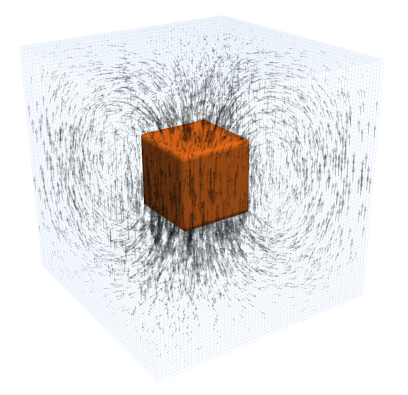
\includegraphics[width=6cm]{images/benchmark_sinker/samm22}\\
{\captionfont Left: Simulation setup for the 3D falling block (SINKER) problem. 
The vectors represent computed flow. Taken from \textcite{fumt11} (2011).
Right: same experiment in \textcite{samm22} (2022). }
\end{center}


%.......................................................
\paragraph{Sinking block results for multiple elements}

The setup is slightly altered: the domain is 512x512km. 
The block has size $L_b\times L_b=128\times 128$km, and is centered
on ($L_x/2,3L_y/4$). Free slip on all sides. Pressure is volume normalised. $|g_y|=10$.
This benchmark is part of \aspect, and can therefore be run with $Q_2\times Q_1$, $Q_2\times P_{-1}$ and $Q_1\times P_0$ elements (although the solver does not converge for the latter at high resolutions).
Velocity and pressure are measured in the middle of the block (in the case of the $Q_1^+\times P_0$ element the 
projected pressure $q$ on the $Q_1$ is used).

As above, the quantity $|v|\eta_1/\delta\rho$velocity is considered, but this time plotted as a function 
of the resolution for a fixed $\eta_2$ and for various element types. The quantity $p/\delta\rho/L_b$
is also plotted:

\begin{center}
\includegraphics[width=7.9cm]{images/benchmark_sinkingblock/eta2_1e18/v.pdf}
\includegraphics[width=7.9cm]{images/benchmark_sinkingblock/eta2_1e18/p.pdf}\\
{\captionfont Results for $\rho_1=0$, $\rho_2=\delta\rho=8$, $\eta_1=10^{21}$ and $\eta_2=10^{18}$}
\end{center}

\begin{center}
\includegraphics[width=7.9cm]{images/benchmark_sinkingblock/eta2_1e22/v.pdf}
\includegraphics[width=7.9cm]{images/benchmark_sinkingblock/eta2_1e22/p.pdf}\\
{\captionfont Results for $\rho_1=0$, $\rho_2=\delta\rho=8$, $\eta_1=10^{21}$ and $\eta_2=10^{22}$}
\end{center}

Results obtained with \aspect with $\rho_1=3200$ and $\rho_2=\rho_1+\delta\rho$ are shown here:

\begin{center}
\includegraphics[width=12cm]{images/benchmark_sinkingblock/aspect/v.pdf}
\end{center}


%......................................................
\subsection{The hot blob problem}\label{sec:hotblob}

This is a very similar setup as the 3D sinker from the same authors
with higher but more diffusive variation of viscosity.
The body force is given by $(0, 0, \beta T)$ and
where the temperature field $T$ is defined by $T = \exp  (-\gamma (x^2+y^2+(z-0.3)^2))$ 
with the constant parameters $\beta=10^6$ and $\gamma=200$. 
The temperature-dependent viscosity $\eta = \exp( -\alpha T)$ is employed with the parameter for viscosity
contrast $\alpha$.

\begin{center}
\includegraphics[width=8cm]{images/benchmark_hotblob/fumt11}\\
{\captionfont Simulation setting of BLOB problem. Isosurface and vectors represent temperature field \\and computed flow respectively. Taken from \cite{fumt11}}
\end{center}

%...........................................................
\subsection{The punch/indentor problem in 2D} \label{sec:punch}

The punch benchmark is one of the few boundary value problems involving plastic solids 
for which there exists an exact solution. 
Such solutions are usually either for highly simplified geometries (spherical or axial 
symmetry, for instance) or simplified material models (such as rigid plastic solids) \cite{kacha04}.

In this experiment, a rigid punch indents a rigid plastic half space; the slip line field theory gives 
exact solutions as shown hereunder:

\begin{center}
\includegraphics[width=6cm]{images/benchmark_punch/thfb08}\\
{\captionfont Two-dimensional rigid punch indenting a rigid
plastic half space. (a) Prandtl's rigid plastic solution; (b)
Hill's solution. Taken from \cite{thfb08}}
\end{center}

The plane strain formulation of the equations and the detailed solution to the problem 
were derived in the Appendix of \cite{thfb08} and are also presented in \cite{gepd98} 
and in \cite[Chapt.6]{bower2009}.
The two dimensional punch problem has been extensively studied numerically for the past 40 years 
\cite{zihl75,prlo90,zihp95,ziph95,chpe01,chan99,huhy99,yuti06,bufs08,raab07,gltf18} and has been used to draw a parallel with the tectonics of eastern China in the context of the 
India-Eurasia collision \cite{tamo76,mota77,engl82} or the European Alps \cite{repe97}.
It is also worth noting that it has been carried out in one form or another in series of 
analogue modelling articles concerning the same region, with a rigid indenter colliding with a rheologically 
stratified lithosphere \cite{tapl82,peta88,daco88,jodc90}.


\begin{center}
a)\includegraphics[width=5cm]{images/benchmark_punch/gps}
b)\includegraphics[width=5cm]{images/benchmark_punch/img5}
c)\includegraphics[width=5cm]{images/benchmark_punch/img7}\\
d)\includegraphics[width=5cm]{images/benchmark_punch/img6}
e)\includegraphics[width=5cm]{images/benchmark_punch/img8}
f)\includegraphics[width=5cm]{images/benchmark_punch/img11}\\
{\captionfont b,c) Model by Tapponnier \etal (1982) \cite{tapl82} or 
Peltzer \& Tapponnier (1988) \cite{peta88}. Not sure about source for other figures.}
\end{center}


 
Numerically, the one-time step punch experiment is performed on a two-dimensional
domain of purely plastic von Mises material. 
Given that the von Mises rheology yield criterion does not depend on pressure, the density of the material and/or the gravity vector is set to zero. Sides are set to free slip boundary conditions, the bottom to no slip, while a vertical velocity $(0,-v_p)$ is prescribed at the top boundary for nodes whose $x$ coordinate is within $[L_x/2-\delta/2,L_x/2+\delta/2]$. 

The analytical solution predicts that the angle of the shear bands stemming from the sides of the punch 
is $\pi/4$, that the pressure right under the punch is $1+\pi$, 
and that the velocity of the rigid blocks on each side of the punch is $v_p/\sqrt{2}$ 
(this is simply explained by invoking conservation of mass).


\begin{center}
\includegraphics[width=10cm]{images/benchmark_punch/gltf18}\\
{\captionfont The punch benchmark results after 500 nonlinear iterations for a rough punch (left column) 
and a smooth punch (right column). (a,f) Viscosity field with analytical slip lines. 
(b,g) Strain rate norm $\dot\varepsilon_e$ with measured shear band angles. 
(c,h) Velocity magnitude with velocity vectors along the surface of the domain.
(d,i) Pressure field. (e,j) Pressure along the surface of the domain (colored line) and analytical 
solution values $\pi + 1$ and 1 (grey lines). Taken from \cite{gltf18}}
\end{center}

\begin{remark}
This benchmark is often mentioned or used in the context of bearing capacity, footings, 
limit state design/analysis \cite{mich01,zhll03,gour04,gork06,lesk05,shls03}.
\end{remark}


%................................................................................
\subsection{Driven cavity with analytical solution} \label{sec:ldc_anal}

This comes from Elman \etal \cite{elsw}(section 3.1.4)\footnote{actually, not?}. The velocity is prescribed to be
\[
{\vec v}=(2y(1-x^2) ; -2x(1-y^2) )
\]
on the domain $\Omega=[-1:1]\times[-1:1]$. The strainrate tensor is given by:
\[
\dot{\bm \varepsilon}=
\left(
\begin{array}{cc}
-4xy & -x^2+y^2  \\
-x^2+y^2 & 4xy   
\end{array}
\right)
\]
The Stokes equation is then:
\begin{eqnarray}
-\frac{\partial p}{\partial x} + 2\eta ( -4y + 2y ) &=& \rho g_x \\
-\frac{\partial p}{\partial y} + 2\eta ( -2x + 4x ) &=& \rho g_y
\end{eqnarray}
where we assume the viscosity $\eta=1$ to be constant in space.
Assuming $g_x=0$, the first equation is
\[
\frac{\partial p}{\partial x} = - 4 y
\]
i.e.
\[
p(x,y)= -4  y x +f(y)
\]
Inserting this in the second equation:
\[
4  x - f'(y) + 4 x  = \rho g_y
\]
or,
\[
-f'(y) + 8  x  = \rho g_y
\]
Assuming $g_y=-1$, we get $\rho=-8x$ and then $f'(y)=0$ so $f(y)=C$ where $C$
is a constant.
Finally the pressure is given by:
\[
p(x,y)=-4  y x + C
\]
We add the following requirement: $\int_\Omega p(x,y) d\Omega =0$ so that $C=0$.

\begin{center}
\includegraphics[width=6cm]{images/benchmark_ldc_anal/velo}
\includegraphics[width=6cm]{images/benchmark_ldc_anal/press}
\end{center}

\begin{eqnarray}
\upnu_{rms}^2 
&=& \frac{1}{\Omega} \int_\Omega (u^2+v^2) d\Omega \nonumber\\
&=& \frac{1}{4} \int_{-1}^{+1}\int_{-1}^{+1} (u^2+v^2) dxdy \nonumber\\
&=& \frac{1}{4} \int_{-1}^{+1}\int_{-1}^{+1} [ 4y^2(1-x^2)^2 + 4x^2(1-y^2)^2   ] dxdy \nonumber\\
&=& \int_{-1}^{+1}\int_{-1}^{+1} [ y^2(1-x^2)^2 + x^2(1-y^2)^2   ] dxdy \nonumber\\
&=& \int_{-1}^{+1}\int_{-1}^{+1} [ y^2(1-2x+x^2) + x^2(1-2y+y^2)  ] dxdy \nonumber\\
&=& \int_{-1}^{+1}\int_{-1}^{+1} y^2 dxdy
+ \int_{-1}^{+1}\int_{-1}^{+1} 2 x^2 y^2 dxdy
+ \int_{-1}^{+1}\int_{-1}^{+1} x^2 dxdy\nn\\
&=& 2  \frac23 + 2 \frac23\frac23 + 2 \frac23 \nn\\
&=& \frac{32}{9} \nn\\
&=& 3.5555
\end{eqnarray}

We can reformulate the benchmark in the unit square $\Omega=[0:1]\times[0:1]$.

\begin{eqnarray}
u(x,y) &=&  (2y-1)x(1-x) \nn\\
v(x,y) &=& - (2x-1)y(1-y) \nn
\end{eqnarray}

Then 
\begin{eqnarray}
\dot\varepsilon_{xx}(x,y) &=& (2y-1)(1-2x) \nn\\
\dot\varepsilon_{xy}(x,y) &=&  x(1-x)  - y(1-y)  \nn\\
\dot\varepsilon_{yy}(x,y) &=& - (2x-1)(1-2y)  \nn
\end{eqnarray}
We of course recover 
\[
\dot\varepsilon_{xx}(x,y) + \dot\varepsilon_{yy}(x,y) = 0
\]
The Stokes equation is then:
\begin{eqnarray}
-\frac{\partial p}{\partial x} + 2\eta (-2(2y-1)-(1-2y)  ) &=& \rho g_x \nn\\
-\frac{\partial p}{\partial y} + 2\eta ((1-2x)+2(2x-1)  ) &=& \rho g_y \nn
\end{eqnarray}
or
\begin{eqnarray}
-\frac{\partial p}{\partial x} + 2\eta (1-2y) &=& \rho g_x \nn\\
-\frac{\partial p}{\partial y} - 2\eta (1-2x) &=& \rho g_y \nn
\end{eqnarray}
where we assume the viscosity $\eta=1$ to be constant in space.
Assuming $g_x=0$, the first equation is
\[
\frac{\partial p}{\partial x} =  2 (1-2y)
\]
i.e.
\[
p(x,y) = 2 x (1-2y) + f(y)
\]
Inserting this in the second equation:
\[
4 x - f'(y) - 2 (1-2x)   = \rho g_y
\]
Assuming $g_y=-1$, then
\[
8 x -2  - f'(y)  = \rho 
\]
we set $\rho(x,y)= 8x-2$ and then $f'(y)=0$ so $f(y)=C$ where $C$
is a constant.
Finally the pressure is given by:
\[
p(x,y)= 2 x (1-2y) + C
\]
We add the following requirement: $\int_\Omega p(x,y) d\Omega =0$ 
\[
\int_{0}^1 \int _0^1 p(x,y) = 0
\Rightarrow 
\int_{0}^1 \int _0^1 [ 2 x (1-2y) + C] = 0
\]
so that $C=0$.

We also find $\upnu_{rms}=\frac{1}{\sqrt{45}}\simeq 0.1490711985$



%................................................................................
\subsection{Viscous flow around a cylinder in 2D and 3D } \label{sec:flowcyl}

There are many variants of this problem: 2D in Turek \cite{turek}, 3D in John \cite{john02}.
Many studies focus on Navier-Stokes flow since the cylinder generates
vortices at high Reynolds numbers. Steady state solutions at low Re are shown 
here\footnote{\url{up of the test and data measurement}}.
Note the interesting benchmark for 2D visco-elastic flow in Beuchert \& Podlachikov \cite{bepo10}.

\begin{center}
\includegraphics[width=8cm]{images/benchmark_flow_cylinder/turek}
\includegraphics[width=6cm]{images/benchmark_flow_cylinder/john02}\\
{\captionfont Left: taken from Turek \cite{turek}; Right: taken from John \cite{john02}}
\end{center}

\Literature: Tachibana \& Iemoto (1987) \cite{taie87}
Sch\"afer \& Turek (1996) \cite{sctu96}


%................................................................................
\subsection{Heat flow around a cylinder} \label{sec:hfcyl}

The domain is a 2D Cartesian box of size 8x4.
The Stokes equations are not solved and the following velocity is prescribed:
\begin{eqnarray}
u(x,y)&=& U_\infty \left(  1-\frac{x^2-y^2}{(x^2+y^2)^2}  \right) \\
v(x,y)&=& -2U_\infty \frac{xy}{(x^2+y^2)^2}
\end{eqnarray}
Boundary conditions are as follows:
$T=0$ is imposed at the top and bottom of the domain. 
$T=1$ is imposed inside a disc centered at (2,2) with radius 1.  
Further: $k=0.01$, $C_p=1$, $\rho=1$, CFL number is 0.1.

\begin{center}
\includegraphics[width=5cm]{images/benchmark_heatcyl/u}
\includegraphics[width=5cm]{images/benchmark_heatcyl/w}
\includegraphics[width=5cm]{images/benchmark_heatcyl/vel}
\end{center}

\begin{center}
\includegraphics[width=5cm]{images/benchmark_heatcyl/temper_0000}
\includegraphics[width=5cm]{images/benchmark_heatcyl/temper_0020}
\includegraphics[width=5cm]{images/benchmark_heatcyl/temper_0040}\\
\includegraphics[width=5cm]{images/benchmark_heatcyl/temper_0060}
\includegraphics[width=5cm]{images/benchmark_heatcyl/temper_0080}
\includegraphics[width=5cm]{images/benchmark_heatcyl/temper_0150}\\
{\captionfont Time evolution of the temperature field.
Results obtained with \elefant (unpublished)}
\end{center}

This is carried out in \stone 65.

%................................................................................
\subsection{Thermal diffusion of half-cooling space} \label{sec:hcsp}

This is a simple 1D experiment which solution is (for instance) available 
in Turcotte \& Schubert \cite{tusc} and is also presented in Choi \etal \cite{chtl13}.

The domain is 100km deep. $T_0=$0\degree C is prescribed a the surface and 
$T_m=$1300\degree C is prescribed at the bottom. The initial temperature is $T(y)=1300$\degree C.
The material is characterised by $\rho=1000$kg/m$^3$, $C_p=1000$J/kg/K, 
$k=1$J/m/K. The time-dependent solution is given by:
\begin{equation}
T(y,t)=T_0 + (T_0-T_m) \text{erf} \left( \frac{y}{2\sqrt{k t /\rho C_p}}  \right)
\end{equation}

\begin{center}
\includegraphics[width=6cm]{images/benchmark_hcsp/chtl13}\\
{\captionfont Thermal diffusion of half space cooling plate.
The temperature profiles in the analytical solution at 1, 5,
and 15 Myrs are plotted in solid lines. The results from
DynEarthSol2D are plotted in circles. Taken from \cite{chtl13}}
\end{center}


%................................................................................
\subsection{Laplace equation on a semi infinite plate} \label{sec:lapplate}
\input{benchmark_laplace_plate}

%................................................................................
\subsection{Slab detachment benchmark} \label{sec:slabdetach}

\Literature: Schmeling (2011) \cite{schm11}, \aspect manual \cite{aspectmanual}, Glerum \etal \cite{gltf18}, 
\stone 26.

\begin{center}
\includegraphics[width=6cm]{images/benchmark_slabdetach/gltf18}\\
{\captionfont The detachment benchmark model setup of Schmalholz \cite{schm11}: 
a symmetric system of nonlinear viscous lithosphere with a vertical slab extending into a linear 
viscous mantle. The top and bottom boundaries are free slip, while the vertical boundaries are no slip.
Taken from \cite{gltf18}.}
\end{center}

%................................................................................
\subsection{Layered flow with viscosity contrast} \label{sec:layfl}

The idea behind this benchmark is to construct an analytical solution to the incompressible
Stokes equation in the case where the viscosity field showcases a 
viscosity contrast at location $y=y_0$ whose amplitude and width can be controlled. 
The viscosity is defined as
\[
\eta(y)=\frac{1}{\frac{1}{\pi} \tan^{-1} (\frac{y-y_0}{\beta} ) + 1/2 + \epsilon}
\]
where $\beta$ and $\epsilon$ are parameters. 

\begin{center}
\includegraphics[width=7cm]{images/benchmark_layeredflow/viscosityA}
\includegraphics[width=7cm]{images/benchmark_layeredflow/viscosityB}\\
\includegraphics[width=7cm]{images/benchmark_layeredflow/viscosityC}
\includegraphics[width=7cm]{images/benchmark_layeredflow/viscosityD}\\
{\captionfont Viscosity profiles for different values of $\beta$ and $\epsilon$ 
for $y_0=1/3$.
When $\beta$ is very large, the viscosity 
essentially converges to $\sim (1/2 + \epsilon)^{-1}$. 
$\beta$ controls the width of the transition while $\epsilon$ controls the amplitude 
of the viscosity variation.}
\end{center}

The flow is assumed to take place in an infinitely long pipe (in the horizontal direction)
and bound by 
$y=-1$ and $y+1$.
At the bottom we impose $v_x(y=-1)=0$ while we impose $v_x(y=+1)=1$ at the top.
The density is set to 1 while the gravity is set to zero.
Under these assumptions, the flow velocity and pressure fields are given by:
\begin{eqnarray}
v_x(x,y)&=&\frac{1}{2\pi} \left(  -\beta C_1 \log [\beta^2 + (z-y_0)^2]  + 2 (z-y_0)  C_1 \tan^{-1} \frac{z-y_0}{\beta} + \pi (1+2\epsilon) z C_1  + C_2 \right) \nonumber\\
v_y(x,y) &=& 0 \nonumber\\ 
p(x,y) &=& 0 
\end{eqnarray}
where $C_1$ and $C_2$ are integration constants:
\begin{eqnarray}
C_1 &=& 2\pi \left[ 
 \beta  \log [\beta^2 + (1+y_0)^2]  -  2(1+y_0) \tan^{-1} \frac{1+y_0}{\beta} 
-\beta  \log [\beta^2 + (1-y_0)^2]  +  2(1-y_0) \tan^{-1} \frac{1-y_0}{\beta} + 2\pi (1+2\epsilon)   \right]^{-1} \nonumber\\
C_2 &=&  \left[ \beta  \log [\beta^2 + (1+y_0)^2]  -  2(1+y_0) \tan^{-1} \frac{1+y_0}{\beta} + \pi(1+2\epsilon) \right]C_1, 
\end{eqnarray}

\begin{center}
\includegraphics[width=7cm]{images/benchmark_layeredflow/layeredflow_vel}
\includegraphics[width=7cm]{images/benchmark_layeredflow/layeredflow_viscosity}\\
{\captionfont Velocity and viscosity fields}
\end{center}

\paragraph{Analytical derivations} 
The flow takes place in the horizontal direction and is infinite in the this direction too so that:
\[
\vec\upnu=(u(y),0)
\]
The strain rate tensor is then given by:
\[
\dot{\bm \varepsilon}=
\frac{1}{2}
\left(
\begin{array}{cc}
0 & du/dy \\
du/dy & 0
\end{array}
\right)
\]
The momentum equation then becomes:
\[
{\vec \nabla} \cdot (2 \eta \dot{\bm \varepsilon} ) -{\vec \nabla}p 
=
{\vec \nabla} \cdot \left[ \eta(y) 
\left(
\begin{array}{cc}
0 & du/dy \\
du/dy & 0
\end{array}
\right)
\right] -{\vec \nabla}p 
= \rho {\vec g}
\]
On the vertical axis, when the gravity is zero, the equation is automatically verified when the 
pressure is zero.
On the horizontal axis:
\[
\frac{d}{dy} \left(\eta(y) \frac{du}{dy} \right) = 0
\]
Then 
\[
\eta(y) \frac{du}{dy}  = C_1
\]
or,
\[
\frac{du}{dy}  = \frac{C_1}{\eta(y)} = C_1 \left(\frac{1}{\pi} \tan^{-1} \frac{y-y_0}{\beta} 
+ 1/2 + \epsilon\right)
\]
so that the velocity is given by:
\[
u(y) = \frac{1}{\pi} ( y \tan^{-1}((y-y_0)/\beta) - y_0 \tan^{-1}((y-y_0)/\beta)  
-0.5* \beta \log (\beta^2 + y^2 - 2 y y_0 +y_0^2) + \pi y (\epsilon +0.5)) 
\]

\[
u(z)=\frac{1}{2\pi} \left(  -\beta C_1 \log [\beta^2 + (z-y_0)^2]  + 2 (z-y_0)  C_1 \tan^{-1} \frac{z-y_0}{\beta} + \pi (1+2\epsilon) z C_1  + C_2 \right)
\]
where $C_1$ and $C_2$ are integration constants.
I wish to impose $u(z=-1)=0$ and $u(z=+1)=1$:
\[
\frac{1}{2\pi} \left(  -\beta C_1 \log [\beta^2 + (-1-y_0)^2]  + 2 (-1-y_0)  C_1 \tan^{-1} \frac{-1-y_0}{\beta} - \pi (1+2\epsilon)  C_1  + C_2 \right) = 0
\]
\[
\frac{1}{2\pi} \left(  -\beta C_1 \log [\beta^2 + (1-y_0)^2]  + 2 (1-y_0)  C_1 \tan^{-1} \frac{1-y_0}{\beta} + \pi (1+2\epsilon)  C_1  + C_2 \right) = 1
\]
or,
\[
 -\beta C_1 \log [\beta^2 + (-1-y_0)^2]  + 2 (-1-y_0)  C_1 \tan^{-1} \frac{-1-y_0}{\beta} - \pi (1+2\epsilon)  C_1  + C_2 = 0
\]
\[
 -\beta C_1 \log [\beta^2 + (1-y_0)^2]  + 2 (1-y_0)  C_1 \tan^{-1} \frac{1-y_0}{\beta} + \pi (1+2\epsilon)  C_1  + C_2 = 2\pi
\]
or,
\[
 -\beta C_1 \log [\beta^2 + (-1-y_0)^2]  + 2 (1+y_0)  C_1 \tan^{-1} \frac{1+y_0}{\beta} - \pi (1+2\epsilon)  C_1  + C_2 = 0
\]
\[
 -\beta C_1 \log [\beta^2 + (1-y_0)^2]  + 2 (1-y_0)  C_1 \tan^{-1} \frac{1-y_0}{\beta} + \pi (1+2\epsilon)  C_1  + C_2 = 2\pi
\]
or,
\[
-\beta C_1 \log (\beta^2 + (1+y_0)^2)  +  2(1+y_0)C_1 \tan^{-1} ((1+y_0)/\beta) - \pi (1+2\epsilon)  C_1  +C_2  = 0
\]
\[
-\beta C_1 \log (\beta^2 + (1-y_0)^2)  +  2(1-y_0)C_1 \tan^{-1} ((1-y_0)/\beta) + \pi (1+2\epsilon)C_1  +C_2  = 2\pi
\]
I can now substract the first line from the second line:
\[
\beta C_1 \log (\beta^2 + (1+y_0)^2)  -  2(1+y_0)C_1 \tan^{-1} ((1+y_0)/\beta)  
-\beta C_1 \log (\beta^2 + (1-y_0)^2)  +  2(1-y_0)C_1 \tan^{-1} ((1-y_0)/\beta) + 2\pi (1+2\epsilon)C_1    = 2\pi
\]
i.e.,
\[
C_1= 2\pi \left[ 
 \beta  \log [\beta^2 + (1+y_0)^2]  -  2(1+y_0) \tan^{-1} [\frac{1+y_0}{\beta}] 
-\beta  \log [\beta^2 + (1-y_0)^2]  +  2(1-y_0) \tan^{-1} [\frac{1-y_0}{\beta}] + 2\pi (1+2\epsilon)   \right]^{-1}
\]
and then 
\[
C_2= \beta C_1 \log (\beta^2 + (1+y_0)^2)  -  2(1+y_0)C_1 \tan^{-1} ((1+y_0)/\beta) + \pi(1+2\epsilon) C_1 
\]



%\newpage

%\newpage
%For $\epsilon=0$

%\begin{center}
%\includegraphics[width=15cm]{viscosityA}\\
%\includegraphics[width=5cm]{velocity1}
%\includegraphics[width=5cm]{velocity3}
%\includegraphics[width=5cm]{velocity5}
%\end{center}

%\newpage
%For $\epsilon=0.1$

%\begin{center}
%\includegraphics[width=15cm]{viscosityB}\\
%\includegraphics[width=5cm]{velocity6}
%\includegraphics[width=5cm]{velocity8}
%\includegraphics[width=5cm]{velocity10}
%\end{center}



\newpage
%................................................................................
\subsection{The annulus convection benchmark \# 1} \label{ss:anconv}
\begin{flushright} {\tiny {\color{gray} benchmark\_annulus\_converction\_benchmark1.tex}} \end{flushright}
%~~~~~~~~~~~~~~~~~~~~~~~~~~~~~~~~~~~~~~~~~~~~~~~~~~~~~~~~~~~~~~~~~~~~~~~~~~~~~~~~~~~~~~~~~~~~~~~~~~

We wish to solve the Stokes equation in an annulus of inner radius $R_1$
and outer radius $R_2$ with the following boundary conditions:
\begin{itemize}
\item Inner boundary: $\upnu_r(R_1,\theta)=0$ 
\item Outer boundary: $\upnu_r(R_2,\theta)=0$ 
\end{itemize}
We then postulate
\[
\upnu_\theta(r,\theta)= f(r) \cos(k\theta)
\]
Note that in the case $k=0$, we recover a constant velocity on the inner and outer boundaries.

The divergence of an incompressible vector field in polar coordinates is
\[
\frac{1}{r} \frac{\partial (r\upnu_r)}{\partial r} + \frac{1}{r} \frac{\partial \upnu_\theta}{\partial \theta} =0
\]
or, 
\[
\frac{\partial (r\upnu_r)}{\partial r} + \frac{\partial \upnu_\theta}{\partial \theta} =0
\]
i.e.,
\[
\frac{\partial (r\upnu_r)}{\partial r} = - \frac{\partial \upnu_\theta}{\partial \theta} = k f(r) \sin(k\theta) 
\]
so 
\[
r\upnu_r(r,\theta) = k \left[ \int f(r) dr \right] \sin(k\theta) 
\]
and finally 
\[
\upnu_r(r,\theta) = k g(r) \sin(k\theta)  
\]
with 
\begin{eqnarray}
g(r)  &=& \frac{1}{r} \int f(r) dr \\
g'(r) &=& -\frac{1}{r^2} \int f(r) dr + \frac{1}{r} f = - \frac{1}{r} g + \frac{1}{r} f = \frac{1}{r}(f-g) 
\end{eqnarray}


The boundary conditions lead to
\[
\upnu_r(r=R_1,\theta) = 
k (\frac{A}{2}R_1 + \frac{B}{R_1} \ln R_1 + \frac{C}{R_1}) \sin(k\theta)  = 0
\]
\[
\upnu_r(r=R_2,\theta) = 
k (\frac{A}{2}R_2 + \frac{B}{R_2} \ln R_2 + \frac{C}{R_2}) \sin(k\theta)  = 0
\]
This has to be valid $\forall \theta$, so 
%\[
%\frac{A}{2}R_1^2 + B \ln R_1 - 1 =0 
%\]
%\[
%\frac{A}{2}R_2^2 + B \ln R_2 - 1 = 0
%\]
%or, 
\[
\frac{A}{2}R_1^2 + B \ln R_1 =-C
\quad\quad {\rm and} \quad\quad
\frac{A}{2}R_2^2 + B \ln R_2 =-C
\]
leading to 
\[
\frac{A}{2}+ \frac{B}{R_1^2} \ln R_1 =-\frac{C}{R_1^2}
\quad\quad {\rm and} \quad\quad
\frac{A}{2}+ \frac{B}{R_2^2} \ln R_2 =-\frac{C}{R_2^2}
\]
and finally 
\[
B = -C \frac{R_2^2-R_1^2}{R_2^2 \ln R_1 - R_1^2 \ln R_2}
\]
Likewise
\[
\frac{A}{2}R_1^2 + B \ln R_1 = -C
\quad\quad {\rm and} \quad\quad
\frac{A}{2}R_2^2 + B \ln R_2 = -C
\]
yields
\[
\frac{A}{2 \ln R_1}R_1^2 + B  = -\frac{C}{\ln R_1}
\quad\quad {\rm and} \quad\quad
\frac{A}{2 \ln R_2}R_2^2 + B  = -\frac{C}{\ln R_2}
\]
or, 
\[
\frac{A}{2 \ln R_1}R_1^2 - \frac{A}{2 \ln R_2}R_2^2  =  -C (\frac{1}{\ln R_1} - \frac{1}{\ln R_2})
\]
\[
A (\frac{R_1^2}{2 \ln R_1} - \frac{R_2^2}{2 \ln R_2})  =  -C (\frac{1}{\ln R_1} - \frac{1}{\ln R_2})
\]
\[
A (\frac{R_1^2 \ln R_2 }{2 } - \frac{R_2^2 \ln R_1 }{2} )  = -C( \ln R_2 - \ln R_1)
\]
finally
\[
A = -C\frac{2(\ln R_2 - \ln R_1)} { R_1^2 \ln R_2  - R_2^2 \ln R_1}    
= -C\frac{2(\ln R_1 - \ln R_2)} { R_2^2 \ln R_1  - R_1^2 \ln R_2}    
\]


We set ${\vec g}=-g_r {\vec e}_r$.
Stokes equation in Polar coordinates (p284 of Schubert, Turcotte and Olson book):
\begin{itemize}
\item 
$r$-component:
\[
\eta \left[ \nabla^2 \upnu_r - \frac{\upnu_r}{r^2} - \frac{2}{r^2} \frac{\partial \upnu_\theta}{\partial \theta}  \right]
+
\frac{\eta}{3} \frac{\partial}{\partial r} \left[ \frac{1}{r}\frac{\partial (r \upnu_r)}{\partial r} 
+ \frac{1}{r} \frac{\partial \upnu_\theta}{\partial \theta}  \right]
-\frac{\partial p}{\partial r} - \rho g_r = 0
\]
The second term between brackets in the divergence of the velocity field so it is equal to zero in our case. We end up with 
\[
\eta \left[ \nabla^2 \upnu_r - \frac{\upnu_r}{r^2} - \frac{2}{r^2} \frac{\partial u_\theta}{\partial \theta}  \right]
-\frac{\partial p}{\partial r} - \rho g_r = 0
\]
\item 
$\theta$-component:
\[
\eta \left[ \nabla^2 \upnu_\theta +\frac{2}{r^2} \frac{\partial \upnu_r}{\partial \theta} - \frac{\upnu_\theta}{r^2} \right]
+
\frac{\eta}{3} \frac{1}{r} \frac{\partial }{\partial \theta} 
\left[
\frac{1}{r}\frac{\partial (r \upnu_r)}{\partial r} + \frac{1}{r} \frac{\partial \upnu_\theta}{\partial \theta} 
\right]
- \frac{1}{r} \frac{\partial p}{\partial \theta}  = 0
\]
The second term between brackets in the divergence of the velocity field so it is equal to zero in our case. We end up with 
\[
\eta \left[ \nabla^2 \upnu_\theta +\frac{2}{r^2} \frac{\partial \upnu_r}{\partial \theta} - \frac{\upnu_\theta}{r^2} \right]
- \frac{1}{r}\frac{\partial p}{\partial \theta} = 0
\]
\end{itemize}
In both equations, $\nabla^2$ represents the Laplacian of a scalar quantity:
\[
\nabla^2 = \frac{\partial^2}{\partial r^2} + \frac{1}{r} \frac{\partial }{\partial r} + \frac{1}{r^2} \frac{\partial^2 }{\partial \theta^2}
\]
We can then write the two momentum equations for an incompressible Stokes flow in polar coordinates:
\[
\eta \left[ 
\frac{\partial^2 \upnu_r}{\partial r^2} + \frac{1}{r} \frac{\partial \upnu_r}{\partial r} 
+ \frac{1}{r^2} \frac{\partial^2 \upnu_r}{\partial \theta^2}
- \frac{\upnu_r}{r^2} - \frac{2}{r^2} \frac{\partial \upnu_\theta}{\partial \theta}  \right]
-\frac{\partial p}{\partial r} - \rho g_r = 0
\]
\[
\eta \left[ 
\frac{\partial^2 \upnu_\theta}{\partial r^2} + \frac{1}{r} \frac{\partial \upnu_\theta}{\partial r} 
+ \frac{1}{r^2} \frac{\partial^2 \upnu_\theta}{\partial \theta^2}
+\frac{2}{r^2} \frac{\partial \upnu_r}{\partial \theta} - \frac{\upnu_\theta}{r^2} \right]
- \frac{1}{r}\frac{\partial p}{\partial \theta}  = 0
\]
We can further choose $\eta=1$, so that 
\begin{equation}
\frac{\partial^2 \upnu_r}{\partial r^2} + \frac{1}{r} \frac{\partial \upnu_r}{\partial r} 
+ \frac{1}{r^2} \frac{\partial^2 \upnu_r}{\partial \theta^2}
- \frac{\upnu_r}{r^2} - \frac{2}{r^2} \frac{\partial \upnu_\theta}{\partial \theta} 
-\frac{\partial p}{\partial r} - \rho g_r = 0
\label{eq1}
\end{equation}
\begin{equation}
\frac{\partial^2 \upnu_\theta}{\partial r^2} + \frac{1}{r} \frac{\partial \upnu_\theta}{\partial r} 
+ \frac{1}{r^2} \frac{\partial^2 \upnu_\theta}{\partial \theta^2}
+\frac{2}{r^2} \frac{\partial \upnu_r}{\partial \theta} - \frac{\upnu_\theta}{r^2} 
-\frac{1}{r}\frac{\partial p}{\partial \theta} = 0
\label{eq2}
\end{equation}

Let us define $f(r)= Ar+B/r$. We then have 
\begin{eqnarray}
 \frac{\partial^2 f}{\partial r^2} + \frac{1}{r} \frac{\partial f}{\partial r} - \frac{f}{r^2} 
&=& A \left( \frac{\partial^2 r}{\partial r^2} + \frac{1}{r} \frac{\partial r}{\partial r} - \frac{1}{r}\right) 
+ B \left(\frac{\partial^2 r^{-1}}{\partial r^2} + \frac{1}{r} \frac{\partial r^{-1}}{\partial r}  - \frac{1}{r^3}\right) =0
%\nn\\
%&=& \frac{A}{r} + B \left( \frac{2}{r^3} - \frac{1}{r^3}  \right) - \frac{A}{r} -  \frac{B}{r^3}  \nn\\
%&=& 0 \nn
\end{eqnarray}
Eq. (\ref{eq2}) simplifies to:
\[
\frac{1}{r^2} \frac{\partial^2 \upnu_\theta}{\partial \theta^2}
+\frac{2}{r^2} \frac{\partial \upnu_r}{\partial \theta} 
-\frac{1}{r}\frac{\partial p}{\partial \theta} = 0
\]
We have 
\[
\frac{1}{r^2} \frac{\partial^2 \upnu_\theta}{\partial \theta^2}
=
-k^2\frac{f(r)}{r^2} \cos (k \theta)  %= -\frac{k^2}{r^2} v_\theta
\quad\quad {\rm and} \quad\quad
\frac{2}{r^2} \frac{\partial \upnu_r}{\partial \theta} 
=
\frac{2k^2}{r^2} g(r)  \cos(k \theta) 
\]
so 
\[
\frac{1}{r}
\frac{\partial p}{\partial \theta} = 
-\frac{k^2}{r^2}f(r) \cos (k \theta) 
+ 
\frac{2k^2}{r^2} g(r)  \cos(k \theta) 
= k^2\left(  \frac{2g(r)-f(r)}{r^2} \right) \cos(k \theta)
\]
and then 
\[
\frac{\partial p}{\partial \theta} = 
 k^2\left(  \frac{2g(r)-f(r)}{r} \right) \cos(k \theta)
\]
This can be integrated with respect to $\theta$:
\[
p(r,\theta)= k\left(  \frac{2g(r)-f(r)}{r} \right) \sin(k \theta) +  l(r)
= k h(r) \sin(k \theta) + l(r)
\]
where $h(r) = \frac{1}{r}(2g(r)-f(r))$.
We can turn to Eq.(\ref{eq1}). 
\begin{eqnarray}
\rho g_r 
&=& 
 \frac{\partial^2 \upnu_r}{\partial r^2} 
+ \frac{1}{r} \frac{\partial \upnu_r}{\partial r} 
+ \frac{1}{r^2} \frac{\partial^2 \upnu_r}{\partial \theta^2}
- \frac{\upnu_r}{r^2} 
- \frac{2}{r^2} \frac{\partial \upnu_\theta}{\partial \theta} 
-\frac{\partial p}{\partial r}  \nn\\
&=& 
+ k g''(r) \sin (k \theta) 
+ k \frac{g'(r)}{r} \sin (k \theta) 
- k^3 \frac{g(r)}{r^2} \sin(k\theta) 
- k \frac{g(r)}{r^2} \sin(k \theta) 
+ k \frac{2f(r)}{r^2}  \sin(k \theta)
- k h'(r) \sin(k \theta) 
- l'(r) \nn\\
&=& k \sin(k\theta)
\left[ g'' + \frac{g'}{r} - \frac{k^2 g }{r^2} - \frac{g}{r^2} + \frac{2f}{r^2} - h'  \right] - l'(r) \nn\\
&=& k \sin(k\theta)
\left[ g'' + \frac{g'}{r} - \frac{k^2 g }{r^2} - \frac{g}{r^2} + \frac{2f}{r^2} + \frac{1}{r^2} (2g-f) - \frac{1}{r} (2g'-f')   \right] - l'(r) \nn\\
&=& k \sin(k\theta)
\left[ g'' + \frac{g'}{r} ( 1 - 2) - \frac{g}{r^2} (k^2 + 1 -2)  + \frac{f}{r^2}  (2-1)  + \frac{f'}{r}   \right] - l'(r) \nn\\
&=& k \sin(k\theta)
\left[ g'' - \frac{g'}{r}  - \frac{g}{r^2} (k^2 - 1)  + \frac{f}{r^2}   + \frac{f'}{r}   \right] - l'(r) 
\end{eqnarray}

We can further choose $g_r=1$. Note that when $k=0$, we have $\rho = -l'(r) $.
We then choose $l'(r)=-\rho_0$ so that the $k$-dependent term can be seen as a density perturbation:
\[
\rho = k \sin (k \theta) \aleph(r) + \rho_0
\]
with 
\[
\aleph(r) = 
g'' + \frac{g'}{r} ( 1 - \frac{2}{r}) - \frac{g}{r^2} (k^2 + 1 -\frac{4}{r}) + \frac{2f}{r^2}  (1-\frac{1}{r}) + \frac{f'}{r^2}  
\]
and
\begin{eqnarray}
f(r)   &=& Ar +\frac{B}{r}\\
f'(r)  &=& A - \frac{B}{r^2}\\
g(r)   &=& \frac{A}{2}r  +  \frac{B}{r} \ln r - \frac{1}{r}\\
g'(r)  &=& \frac{A}{2}  +  \frac{B}{r^2} (1-\ln r)   + \frac{1}{r^2}\\
g''(r) &=& -\frac{2B}{r^3} (1-\ln r)  - B \frac{1}{r^3}  - \frac{2}{r^3} = - \frac{B}{r^3} (3 - 2 \ln r ) 
\end{eqnarray}
Finally, the pressure is then given by 
\[
p(r,\theta)= k\left(  \frac{2g-f}{r^2} \right) \sin(k \theta) +  l(r)
= k h(r) \sin(k \theta) + \rho_0 g_r r + Constant
\]
We enforce $p(r=R_2,\theta)=0$ so that 
\[
p(r,\theta)= k\left(  \frac{2g-f}{r^2} \right) \sin(k \theta) +  l(r)
= k h(r) \sin(k \theta) + \rho_0 g_r (r-R_2) 
\]

%..........................................
\paragraph{Summary of the previous pages}:
\begin{eqnarray}
\upnu_\theta(r,\theta) &=& f(r) \cos(k\theta) \\
\upnu_r(r,\theta) &=& g(r) k  \sin(k\theta)  \\
p(r,\theta) &=& k h(r) \sin(k \theta) + \rho_0 g_r (r-R_2)  \\
\rho(r,\theta) &=& k \sin (k \theta) \aleph(r) + \rho_0 \\
A &=& \frac{2(\ln R_1 - \ln R_2)} { R_2^2 \ln R_1  - R_1^2 \ln R_2}    \\
B &=& \frac{R_2^2-R_1^2}{R_2^2 \ln R_1 - R_1^2 \ln R_2} \\
f(r)   &=& Ar +\frac{B}{r} \\
f'(r)  &=& A - \frac{B}{r^2} \\
g(r)   &=& \frac{A}{2}r  +  \frac{B}{r} \ln r - \frac{1}{r} \\
g'(r)  &=& \frac{A}{2}  +  \frac{B}{r^2} (1-\ln r)   + \frac{1}{r^2} \\
g''(r) &=&  - \frac{B}{r^3} (3 - 2 \ln r )  \\
h(r)   &=& \frac{1}{r^2}(2g-f) \\
\aleph(r) &=&  -g'' - \frac{g'}{r} ( 1 - \frac{2}{r}) + \frac{g}{r^2} (k^2 + 1 -\frac{4}{r})  - \frac{2f}{r^2}  (1-\frac{1}{r}) - \frac{f'}{r^2}   
\end{eqnarray}

%..........................................
\paragraph{Averagings of fields}:

\begin{itemize}
\item Average $\upnu_r$ velocity
\[
<\upnu_r(r)> =\frac{1}{2\pi}\int_0^{2\pi} \upnu_r(r,\theta) d\theta
=\frac{1}{2\pi}\int_0^{2\pi}  g(r) k \sin(k \theta) d\theta
=\frac{1}{2\pi}g(r) k \int_0^{2\pi}  \sin(k \theta) d\theta = 0
\]
since $k=0,2,4,...$

\item Average $\upnu_\theta$ velocity
\[
<\upnu_\theta(r)>
=\frac{1}{2\pi}\int_0^{2\pi} \upnu_\theta(r,\theta) d\theta
=\frac{1}{2\pi}\int_0^{2\pi} f(r) \cos(k \theta) d\theta
=\frac{1}{2\pi}f(r)\int_0^{2\pi}  \cos(k \theta) d\theta
=0
\]
since $k=0,2,4,...$

\item Root mean square verage $\upnu_r$ velocity
\begin{eqnarray}
<\upnu_r>_{rms}(r) 
&=& \sqrt{\frac{1}{2\pi} \int_0^{2\pi} \upnu_r^2 d\theta }   \nn\\
&=& \sqrt{\frac{1}{2\pi} g(r)^2 k^2\int_0^{2\pi} \sin^2 (k \theta) d\theta }   \nn\\
&=& \sqrt{\frac{1}{2\pi} g(r)^2 k^2\int_0^{2\pi} \frac{1}{2}(1-\cos (2k\theta)  ) d\theta }   \nn\\
&=& \sqrt{\frac{1}{2\pi} g(r)^2 k^2  \left(\pi - \frac{1}{2}  \int_0^{2\pi} \cos (2k\theta)   d\theta \right) }   \nn\\
&=& \sqrt{\frac{1}{2\pi} g(r)^2 k^2  \left(\pi - \frac{1}{4k} \underbrace{ \int_0^{2k\pi} \cos \alpha   d\alpha}_{=0} \right) }   \nn\\
&=& \frac{k|g(r)|}{\sqrt{2}} 
\end{eqnarray}

\item Root mean square verage $\upnu_\theta$ velocity

\begin{eqnarray}
<\upnu_\theta>_{rms}(r) 
&=& \sqrt{\frac{1}{2\pi} \int_0^{2\pi} \upnu_\theta^2 d\theta }   \nn\\
&=& \sqrt{\frac{1}{2\pi} f(r)^2 \int_0^{2\pi} \cos^2(k \theta) d\theta }  \nn\\
&=& \sqrt{\frac{1}{2\pi} f(r)^2 \int_0^{2\pi}  \frac{1}{2}(1 + \cos (2k\theta))   d\theta }  \nn\\
&=& \sqrt{\frac{1}{2\pi} f(r)^2 \left( \pi + \frac{1}{2} \int_0^{2\pi}   \cos (2k\theta) d\theta \right)  }  \nn\\
&=& \sqrt{\frac{1}{2\pi} f(r)^2 \left( \pi + \frac{1}{4k} \underbrace{\int_0^{4k\pi}   \cos \alpha d\alpha}_{0} \right)  }  \nn\\
&=& \frac{|f(r)|}{\sqrt{2}}
\end{eqnarray}

\item Root mean square velocity $\upnu_{rms}$

\begin{eqnarray}
\upnu_{rms}=\sqrt{\frac{1}{V}\int_V (\upnu_r^2+\upnu_\theta^2)dV   }
\end{eqnarray}

The volume of the domain is given by 
\[
V=\pi(R_2^2-R_1^2)
\]
and the sum
\begin{eqnarray}
(\upnu_r^2+\upnu_\theta^2 )dV 
&=& [(g(r) k  \sin(k\theta))^2+    (f(r) \cos (k\theta))^2] rdrd\theta \nn\\
&=& [g(r)^2r dr] [k^2  \sin^2(k\theta) d\theta ]+    [f(r)^2 r dr] [ \cos^2 (k\theta) d\theta] \nn
\end{eqnarray}

If $k=0$, we have  $\upnu_\theta = f(r)$ and $\upnu_r = 0$ so that 
%=\sqrt{\frac{1}{V}\int_V (v_r^2+v_\theta^2)dV   }
%=\sqrt{\frac{1}{V}\int_0^{2\pi} \int_{R_1}^{R_2} f(r)^2 r dr d\theta   }

\begin{eqnarray}
\upnu_{rms}
&=& \sqrt{ \frac{1}{V}  \int_0^{2\pi}  d\theta  \int_{R_1}^{R_2} f(r)^2 r dr  } \nn\\
&=& \sqrt{ \frac{2 \pi}{\pi(R_2^2-R_1^2) }     \int_{R_1}^{R_2} f(r)^2 r dr  } \nn\\
&=& \sqrt{ \frac{2 }{(R_2^2-R_1^2) }    \int_{R_1}^{R_2} \left( Ar + \frac{B}{r} \right)^2 r dr } \nn\\
&=& \sqrt{ \frac{2 }{(R_2^2-R_1^2) }   \int_{R_1}^{R_2} \left( A^2r^3 + 2ABr + \frac{B^2}{r}  \right) dr } \nn\\
&=& \sqrt{ \frac{2 }{(R_2^2-R_1^2) }    \left[ A^2 \frac{r^4}{4} + ABr^2 + B^2 \ln(r)  \right]_{R_1}^{R_2} } \nn\\
&=& \sqrt{ \frac{2 }{(R_2^2-R_1^2) }  [ \frac{A^2}{4}(R_2^4-R_1^4) + AB (R_2^2-R_1^2) + B^2 (\ln R_2 - \ln R_1) ] }
\end{eqnarray}

If $k\neq 0$ we have
\[
\int_0^{2\pi} k^2  \sin^2(k\theta) d\theta = \frac{1}{2}k^2 \int_0^{2\pi} (1-\cos(k \theta)) d\theta  = \pi k^2
\]
\[
\int_0^{2\pi}   \cos^2(k\theta) d\theta = \frac{1}{2} \int_0^{2\pi} (1+\cos(k \theta)) d\theta  = \pi 
\]
so that 
\[
{\cal V}=\int_0^{2\pi}\int_{R_1}^{R_2} (\upnu_r^2 + \upnu_\theta^2) r dr d\theta =  \pi k^2 \int_{R_1}^{R_2} g(r)^2 r dr + \pi  \int_{R_1}^{R_2} f(r)^2 r dr
\]
\begin{eqnarray}
\int_{R_1}^{R_2} f(r)^2 r dr 
&=&  \int_{R_1}^{R_2} \left( Ar + \frac{B}{r} \right)^2 r dr  \nn\\
&=&  \int_{R_1}^{R_2} \left( A^2r^3 + 2ABr + \frac{B^2}{r}  \right) dr  \nn\\
&=& \left[ A^2 \frac{r^4}{4} + ABr^2 + B^2 \ln(r)  \right]_{R_1}^{R_2}  \nn\\
&=& \frac{A^2}{4}(R_2^4-R_1^4) + AB (R_2^2-R_1^2) + B^2 (\ln R_2 - \ln R_1)
\nn\\
\nn\\
\int_{R_1}^{R_2} g(r)^2 r dr
&=&  \int_{R_1}^{R_2} \left(  \frac{A}{2}r  +  \frac{B}{r} \ln r + \frac{C}{r} \right)^2 r dr  \nn\\
&=&  \int_{R_1}^{R_2} \left(  \frac{A^2}{4}r^2  +  AB \ln r + AC + \frac{2BC}{r^2} \ln r + \frac{B^2}{r^2}(\ln r)^2 + \frac{C^2}{r^2}\right) r dr  \nn\\
&=&  \int_{R_1}^{R_2} \left(  \frac{A^2}{4}r^3  +  AB r \ln r + AC r  + \frac{2BC}{r} \ln r + \frac{B^2}{r}(\ln r)^2 + \frac{C^2}{r}\right)  dr  \nn\\
&=&  \int_{R_1}^{R_2} \left(  \frac{A^2}{4}r^3  + AC r  + \frac{C^2}{r}\right)  dr  + E + F + G\nn\\
&=&  \left[  \frac{A^2}{16}r^4  + \frac{1}{2}AC r^2  + C^2 \ln r \right]_{R_1}^{R_2}    + E + F + G\nn\\
&=&   \frac{A^2}{16} (R_2^4-R_1^4) + \frac{AC}{2} (R_2^2-R_1^2) + C^2 (\ln R_2 - \ln R_1 ) +  E + F + G\nn\\
\end{eqnarray}

\begin{eqnarray}
E
&=&2BC \int_{R_1}^{R_2} \frac{1}{r} \ln r \; dr  \nn\\
&=& BC \int_{\ln R_1}^{\ln R_2} 2X dX  \quad\quad\quad X=\ln r,\;\; dX=dr/r\nn\\  
&=& BC [ X^2 ]_{\ln R_1}^{\ln R_2} \nn\\
&=& BC [ (\ln R_2)^2-(\ln R_1)^2]
\nn\\
\nn\\
F &=&
B^2 \int_{R_1}^{R_2}  \frac{1}{r} (\ln r )^2 dr  \nn\\
&=& B^2 \int_{\ln R_1}^{\ln R_2}  X^2 dX  \quad\quad\quad X=\ln r,\;\; dX=dr/r\nn\\  
&=& \frac{B^2}{3} [ X^3]_{\ln R_1}^{\ln R_2} \nn\\
&=& \frac{B^2}{3} [ (\ln R_2)^3-(\ln R_1)^3] \nn\\
G
&=& AB \int_{R_1}^{R_2}  r \ln r dr  \nn\\
&=& AB [ \frac{1}{2}r^2 \ln r  ]_{R_1}^{R_2} - AB \int_{R_1}^{R_2} \frac{1}{2}r^2 \frac{1}{r} dr \nn\\
&=& \frac{AB}{2} [ R_2^2 \ln R_2 - R_1^2 \ln R_1] - \frac{AB}{2} \int_{R_1}^{R_2} r dr \nn\\
&=& \frac{AB}{2} [ R_2^2 \ln R_2 - R_1^2 \ln R_1] - \frac{AB}{4} [r^2]_{R_1}^{R_2}  \nn\\
&=& \frac{AB}{2} [ R_2^2 \ln R_2 - R_1^2 \ln R_1] - \frac{AB}{4} (R_2^2 - R_1^2) \nn 
\end{eqnarray}


\begin{eqnarray}
{\cal V}/\pi
&=&  \frac{A^2}{4}(R_2^4-R_1^4) + AB (R_2^2-R_1^2) + B^2 (\ln R_2 - \ln R_1) \nn\\
&+&  \frac{A^2k^2}{16} (R_2^4-R_1^4) + \frac{ACk^2}{2} (R_2^2-R_1^2) + C^2 k^2(\ln R_2 - \ln R_1 ) \nn\\
&+& BC k^2[ (\ln R_2)^2-(\ln R_1)^2] \nn\\
&+& \frac{B^2k^2}{3} [ (\ln R_2)^3-(\ln R_1)^3] \nn\\
&+& \frac{ABk^2}{2} [ R_2^2 \ln R_2 - R_1^2 \ln R_1] - \frac{ABk^2}{4} (R_2^2 - R_1^2) \nn\\
&=& \frac{A^2}{16}(4+k^2)(R_2^4-R_1^4) + (\frac{AB}{4}(4-k^2) +\frac{ACk^2}{2}) (R_2^2-R_1^2) \nn\\
&+&  (B^2+C^2 k^2) (\ln R_2 - \ln R_1) \nn\\
&+& BC k^2[ (\ln R_2)^2-(\ln R_1)^2] \nn\\
&+& \frac{B^2k^2}{3} [ (\ln R_2)^3-(\ln R_1)^3] \nn\\
&+& \frac{ABk^2}{2} [ R_2^2 \ln R_2 - R_1^2 \ln R_1] 
\end{eqnarray}

\[
\upnu_{rms} =\sqrt{\frac{1}{V} {\cal V}} = \sqrt{ \frac{1}{2(R_2^2-R_1^2)} \frac{\cal V}{\pi}  }
\]
\end{itemize}



%........................................................
\paragraph{Computing the strain rate and stress tensors}:

Since we know the viscosity, the velocity field and the pressure field, 
we can also compute the full stress tensor 
${\bm \sigma} = - p {\bm 1} + 2 \eta \dot{\bm \varepsilon}$
In this benchmark we have set $\eta=1$ so:
$
{\bm \sigma} = - p {\bm 1} + 2 \dot{\bm \varepsilon}
$
We start with the velocity gradient:
\begin{eqnarray}
{\vec \nabla}{\vec \upnu}
&=&
\left(
\begin{array}{cc}
\frac{\partial \upnu_r}{\partial r}      &  \frac{1}{r}\frac{\partial \upnu_r}{\partial \theta}-\frac{\upnu_\theta}{r}\\\\
\frac{\partial \upnu_\theta}{\partial r} &  \frac{1}{r}\frac{\partial \upnu_\theta}{\partial \theta}+\frac{\upnu_r}{r}
\end{array}
\right) \nonumber\\
&=&
\left(
\begin{array}{cc}
g' k \sin(k\theta)  &  \frac{1}{r} g k^2 \cos(k\theta)  -\frac{1}{r} f \cos(k\theta) \\ \\
f' \cos (k\theta)   &  -\frac{1}{r} f k \sin(k\theta)   +\frac{1}{r} g k \sin(k\theta)
\end{array}
\right) \nonumber\\
&=&
\left(
\begin{array}{cc}
g' k \sin(k\theta)  &  \frac{1}{r} (g k^2 - f) \cos(k\theta) \\ \\
f' \cos (k\theta)   &  \frac{1}{r} ( g-f ) k  \sin(k\theta)
\end{array}
\right) 
\end{eqnarray}
The strain rate is then given by:
\begin{eqnarray}
\dot{\bm \varepsilon} &=&
\frac{1}{2} ( {\bm \nabla}{\bm v} + {\bm \nabla}{\bm v}^T) 
=
\left(
\begin{array}{cc}
g' k \sin(k\theta)  &  \frac{1}{2r} (rf' + g k^2 - f) \cos(k\theta) \\ \\
\frac{1}{2r} (rf' + g k^2 - f) \cos(k\theta)    &  \frac{1}{r} ( g-f ) k  \sin(k\theta)
\end{array}
\right) 
\end{eqnarray}
Let us verify once again that the flow is incompressible:
\[
{\vec \nabla}\cdot{\vec \upnu} 
= g'(r) k \sin(k\theta)  + \frac{1}{r} ( g(r)-f(r) ) k  \sin(k\theta)
= \frac{1}{r} ( r g'(r) + g(r)-f(r) ) k  \sin(k\theta)
=0
\]
since $g'(r)= \frac{1}{r}(f(r)-g(r))$.

I can now write the full stress tensor:
\begin{eqnarray}
{\bm \sigma} = 
- p {\bm 1} + 2 \dot{\bm \varepsilon} 
=
\left(
\begin{array}{cc}
-p + 2 g' k \sin(k\theta)  &  \frac{1}{r} (rf' + g k^2 - f) \cos(k\theta) \\ \\
\frac{1}{r} (rf' + g k^2 - f) \cos(k\theta)    &  -p + \frac{2}{r} ( g-f ) k  \sin(k\theta)
\end{array}
\right) 
\end{eqnarray}

On the boundaries, i.e. $r=R_1$ or $r=R_2$, 
the function $g$ is exactly zero, so that the stress ${\bm \sigma}_b$ 
on the boundaries is given by
\begin{eqnarray}
{\bm \sigma}_b  
=
\left(
\begin{array}{cc}
-p + 2 g' k \sin(k\theta)  &  \frac{1}{r} (rf' - f) \cos(k\theta) \\ \\
\frac{1}{r} (rf'   - f) \cos(k\theta)    &  -p - \frac{2}{r}  f  k  \sin(k\theta)
\end{array}
\right) 
\end{eqnarray}
Furthermore I can use the identity $g'=(f-g)/r$ which simplifies to $g'=f/r$ on the boundaries:
\begin{eqnarray}
{\bm \sigma}_b  
=
\left(
\begin{array}{cc}
-p + 2 \frac{f}{r} k \sin(k\theta)  &  \frac{1}{r} (rf' - f) \cos(k\theta) \\ \\
\frac{1}{r} (rf'   - f) \cos(k\theta)    &  -p - \frac{2}{r}  f  k  \sin(k\theta)
\end{array}
\right)
\end{eqnarray}
Also, $h(r)   = \frac{1}{r}(2g-f) $ simplifies to  $h(r)   = -f/r$ so 
\[
p = k h(r) \sin(k \theta) + \rho_0 g_r (r-R_2)  =
 -k \frac{f}{r} \sin(k \theta) + \rho_0 g_r (r-R_2) 
\]
Finally
\begin{eqnarray}
{\bm \sigma}_b
&=&
\left(
\begin{array}{cc}
 k \frac{f}{r} \sin(k \theta) - \rho_0 g_r (r-R_2) + 2 \frac{f}{r} k \sin(k\theta)  &  \frac{1}{r} (rf' - f) \cos(k\theta) \\ \\
\frac{1}{r} (rf'   - f) \cos(k\theta)    &    k \frac{f}{r} \sin(k \theta) - \rho_0 g_r (r-R_2)   - \frac{2}{r}  f  k  \sin(k\theta)
\end{array}
\right) \nn\\
&=&
\left(
\begin{array}{cc}
 k \frac{3f}{r} \sin(k \theta) - \rho_0 g_r (r-R_2)   &  \frac{1}{r} (rf' - f) \cos(k\theta) \\ \\
\frac{1}{r} (rf'   - f) \cos(k\theta)    &    - k \frac{f}{r} \sin(k \theta) - \rho_0 g_r (r-R_2)  
\end{array}
\right) \nn
\end{eqnarray}
The traction along the normal is given by
\[
{\bm \sigma}_n 
= {\bm \sigma}_b \cdot {\vec n}
= -{\bm \sigma}_b \cdot {\vec e}_{\bm r}
= - \left(
\begin{array}{c}
 k \frac{3f}{r} \sin(k \theta) - \rho_0 g_r (r-R_2) \\  \\
\frac{1}{r} (rf'   - f) \cos(k\theta)    
\end{array}
\right)
\]

\paragraph{Strain rate tensor in Cartesian coordinates} 
The analytical expressions for the strain rate components in polar coordinates 
are:
\begin{eqnarray}
\dot{\varepsilon}_{rr}&=& g'(r) k \sin k\theta \\
\dot{\varepsilon}_{r\theta}=
\dot{\varepsilon}_{\theta r}&=&
\frac{1}{2}\left(
\frac{1}{r} g(r) k^2 \cos k\theta + f'(r) \cos k\theta - \frac{f(r)}{r} \cos k\theta
\right)\\
&=& \frac{1}{2}
\left(
\frac{1}{r} g(r) k^2  + f'(r) - \frac{f(r)}{r} 
\right) \cos k\theta \\
\dot{\varepsilon}_{\theta \theta} 
&=& -\frac{1}{r} k f(r) \sin k\theta + \frac{g(r)}{r}  k \sin k\theta\\
 &=& \frac{g(r)-f(r)}{r} k \sin k\theta
\end{eqnarray}
Their counterparts in Cartesian coordinates are obtained with Eqs.~\eqref{ss:srboth}.

\paragraph{Could we find a steady state temperature field that goes along?}
We can start from the pure advection equation:
\[
\rho C_p \left(\frac{\partial T}{\partial t} + \vec\upnu\cdot \vec\nabla T \right) = 0
\]
At steady state we are left with 
\[
\vec\upnu\cdot \vec\nabla T = 0
\]
I postulate then 
\[
T(r,\theta) = l(r) (\alpha \cos k\theta + \beta \sin k\theta)
\]
Inserting this into the equation above I arrive at the conclusion that $\beta \neq 0$ is a dead end. 
It then simply follows that 
\[
T(r,\theta) = l(r) \cos k\theta 
\]
which yields $T(r,\theta)=r g(r) \cos(k\theta)$. 
and 
\[
\vec\nabla T = ( f(r) \cos k\theta ; - g(r) k \sin k\theta)
\]
I can then plot the temperature gradient (in black) next to the velocity field in red (right figure)
and show that these are indeed always perpendicular:

\includegraphics[height=5cm]{images/benchmark_annulus_conv/T}
\includegraphics[height=5cm]{images/benchmark_annulus_conv/arrows}\\

However, what is deeply puzzling is the fact that the temperature is exactly zero on both 
boundaries (beacuse $g(r)$ is by construction) 
and yet the temperature field is not zero in the middle, in the absence of heat source ... ?












\newpage
%................................................................................
\subsection{The annulus convection benchmark \#2 - no slip bc} \label{ss:anconv2}

\input{mms_annulus2}



%................................................................................
\subsection{Rayleigh-B{\'e}nard convection for silicon oil}

This originates in Jenkins \etal (2014) \cite{jejl14}.

\begin{center}
\includegraphics[width=6cm]{images/benchmark_jejl14/jejl14a}
\includegraphics[width=8cm]{images/benchmark_jejl14/jejl14b}
\end{center}

\newpage
%................................................................................
\subsection{Rayleigh-Taylor experiment of van Keken \etal (1997)} \label{ss:vaks97}
\begin{flushright} {\tiny {\color{gray} benchmark\_vaks97.tex}} \end{flushright}

\vspace{1cm}
\begin{flushright}
Data pertaining to this section are to be found at:
\url{https://github.com/cedrict/fieldstone/tree/master/images/benchmark_vaks97}
\end{flushright}
\vspace{1cm}


This numerical experiment was first presented in \textcite{vaks97} (1997).
It consists of an isothermal Rayleigh-Taylor instability in a two-dimensional box
of size $Lx=0.9142$ and $L_y=1$.

Two Newtonian fluids are present in the system: the buoyant layer is 
placed at the bottom of the box and the interface between both fluids 
is given by 
\begin{equation}
y(x)=0.2+0.02\cos \left( \frac{\pi x}{L_x}  \right)
\end{equation}
The bottom fluid is parametrised by its density $\rho_1=1000$ and 
its viscosity $\eta_1$, while the layer above is parametrised 
by $\rho_2=1010$ and $\eta_2=100$.
This experiment is to be carried out for various viscosity constrasts between the 
two layers, i.e. $\eta_1=\{1,10,100\}$.

No-slip boundary conditions are applied at the bottom and at the top of the box 
while free-slip boundary conditions are applied on the sides.
Gravity is pointing downwards with $|\vec{g}|=10$. 

\begin{center}
\includegraphics[width=4cm]{images/benchmark_vaks97/elefant256_0500.png}
\includegraphics[width=4cm]{images/benchmark_vaks97/elefant256_1000.png}
\includegraphics[width=4cm]{images/benchmark_vaks97/elefant256_1500.png}
\includegraphics[width=4cm]{images/benchmark_vaks97/elefant256_2000.png}\\
{\captionfont Example of time evolution obtained with the \elefant code for 
a 256x256 grid with the particle-in-cell method.\\
{\tiny {\color{gray} in images/benchmark\_vaks97/}}  }
\end{center}

One can measure the following quantities:

\begin{itemize}

\item the root mean square velocity $\upnu_{rms}$ in the domain as a function of time:
\begin{equation}
\upnu_{rms}= \sqrt{ \frac{1}{L_xL_y} \int \int |{\vec \upnu}|^2 dxdy}
\end{equation}

\item the maximum (or local maxima) of the $\upnu_{rms}$ and 
its (their) corresponding time(s)

\item the growth rate of the instability at $t=0$.
From linear stability analysis, the analytical growth rate can 
be calculated \cite{ramb68,ramb81}: 
$\gamma_{th}=0.01094019$, which is valid for an infinitesimal perturbation. 
For each model run, the growth rate $\gamma$ is measured by fitting 
the $\upnu_{rms}$ and/or (?) the maximum 
vertical velocity measurements for a short time $t$. 

\item the total mass of the system $M(t)$ as a function of time. 
Since there is no chemical diffusion in the 
system (pure advection equation) the amount of material in the system 
is to remain constant, and therefore its mass too.
\begin{equation}
M(t) = \int \int \rho(x,y,t) dxdy
\end{equation}
Given the layout described in the previous paragraph, the exact 
analytical initial mass $M_0$ of the system is given by 
\[
M_0=0.9142 \times (0.2 \times 1000 + 0.8\times 1010) = 921.5136
\]
The average density is then 
\[
<\rho>_0=\frac{M_0}{L_xL_y} = 1008
\]
We will then measure the relative mass error as a function of time
\[
\delta M(t) = \frac{M(t)-M_0}{M_0}
\]
which is equal to 
\[
<\delta\rho>(t) = \frac{<\rho>(t)-<\rho>_0}{<\rho>_0}
\]

\item the length of the interface between the fluids. At startup it is given by 
\[
{\cal L}(0) = \int_0^L \sqrt{1 + (dy/dx)^2} dx
\]
with $y(x)=0.2+0.02\cos(\pi x/L)$. Using WolframAlpha, we find
\[
{\cal L}(0)= \frac{L}{\pi} \int_0^\pi \sqrt{1 + 
\left(0.02\frac{\pi}{L}\sin(\pi x /L) \right)^2} dx
\simeq 0.9152786349
\]

\end{itemize}


\paragraph{Instantaneous results}.
Results obtained with \stone~\ref{f25} ($Q_2\times Q_1$ element) 
and \stone~\ref{f93} ($P_2^+\times P_{-1}$ element), 
both with mesh fitted so as to follow the interface between both fluids.

\begin{center}
\begin{tabular}{llp{4cm}p{4cm}p{4cm}}
\hline
            &  & $\eta_1=100$ &  $\eta_1=10$ &  $\eta_1=1$ \\ 
\hline\hline
$\min(u)$   & Stone 25 &  & & -4563.5\\
            & Stone 93 ($P_2^+\times P_{-1}$) &  & &        \\
            & Aspect   &  & &        \\
\hline
$\max(u)$   & Stone 25 &  &  & 1054.03\\
            & Stone 93 ($P_2^+\times P_{-1}$)&  & &        \\
            & Aspect   &  & &        \\
\hline
$\min(v)$   & Stone 25 &  &  & \\
            & Stone 93 ($P_2^+\times P_{-1}$)&  & &        \\
            & Aspect   &  & &        \\
\hline
$\max(v)$   & Stone 25 &  &  & 2070.9\\
            & Stone 93 ($P_2^+\times P_{-1}$)&  & &        \\
            & Aspect   &  & &        \\
\hline
$\max(|v|)$ & Stone 25 & 422.125 & & 4563.67\\
            & Stone 93 ($P_2^+\times P_{-1}$)&  & &        \\
            & Aspect   &  & &        \\
\hline
$v_{rms}$   & Stone 25 & 185.2947 & & 1441.87\\
            & Stone 93 ($P_2^+\times P_{-1}$)&  & &        \\
            & Aspect   &  & &        \\
\hline
$\min(p)$   & Stone 25 & -5048.16 & & -5048.7345\\ 
            & Stone 93 ($P_2^+\times P_{-1}$)&  & &        \\
            & Aspect   &  & &        \\
\hline
$\max(p)$   & Stone 25 & 5033.6947 & & 5032.329\\
            & Stone 93 ($P_2^+\times P_{-1}$)&  & &        \\
            & Aspect   &  & &        \\
\hline
\end{tabular}
\end{center}






\newpage



\begin{center}
\begin{tabular}{lllllll}
\hline
Code & Grid & Method & Growth Rate $\gamma$ & t (max vrms) & max (vrms)   & publication\\
\hline\hline
HS & 41x41 & extrapolated & 0.010996 & 211.1  & 0.0030958 & \cite{vaks97}\\
   & 61x64 & extrapolated & 0.011109 & 209.17 & 0.0031022 & \\
   & 81x81 & extrapolated & 0.011177 & 208.99 & 0.0030916 & \\
\hline
CND & 32x32 && 0.01106 & 208.4 & 0.003092 & \cite{vaks97}\\
    & 48x48 && 0.01106 & 208.5 & 0.0030943 \\
\hline 
SK &   80x80 && 0.01130 & 215.67 & 0.00299279 & \cite{vaks97}\\
   & 120x120 && 0.01127 & 206.38 & 0.0028922 \\
   & 160x160 && 0.01179 & 207.84 & 0.0028970 \\
\hline
PvK & 30x30 & splines & 0.01185 & 213.38 & 0.00300 & \cite{vaks97}\\
    & 50x50 & splines & 0.01198 & 211.81 & 0.003016 \\
    & 80x80 & splines & 0.01207 & 210.75 & 0.003050 \\
    & 100x100 & splines & 0.01211 &  & \\
    & 30x30 & C1 element & 0.01253 & 210.59 & 0.003100 \\
    & 80x80 & C1 element & 0.01225 & 207.05 & 0.003091 \\
\hline
ISMM & 160x160	& &0.00991 & 230.1 & 0.003093	 &\cite{soga01}\\
ISMM & 120x120	& &0.00998 & 226.1 & 0.003133	 &\\
MSOU & 160x160	& &0.00993 & 231.4 & 0.003085	 &\\
MSOU & 120x120	& &0.01020 & 227.6 & 0.003134	 &\\
FSOU & 160x160	& &0.01111 & 217.3 & 0.003118	 &\\
FSOU & 120x120	& &0.01159 & 213.1 & 0.003151	 &\\
\hline
&64x64 	 &5 	&0.01112 	&206.5 	&0.003041 & \cite{taki03} \\
&	 &15 	&0.01117 	&208.8 	&0.003098 & \\
&	 &40 	&0.01115 	&209.9 	&0.003110 & \\
&128x128 &5 	&0.01113 	&208.1 	&0.003079 & \\
&	 &15 	&0.01110 	&208.9 	&0.003097 & \\
&	 &40 	&0.01109 	&209.2 	&0.003102 & \\
\hline
& 120x132 & Level sets & 0.01252 & 211.2 & 0.00301 & \cite{sunh10} \\
\hline
& 67m res. &  & &   215.3  & 0.003106 & \cite{chtl13} \\
& 100m res. & & &   215.28 & 0.003101 & \\
\hline
LaCoDe 	& 1808 elts (10754 dofs)   &&0.01221 & 215& 0.003110 & \cite{demh19} \\
	& 7093 elts (2592 dofs)    &&0.01222 & 212& 0.003080 & \\
	& 17960 elts (107468 dofs) &&0.01222 & 211& 0.003075 & \\
\hline
\end{tabular}\\
{\captionfont Selected Quantities for the Isoviscous Rayleigh-Taylor problem.
HS: FDM, stream function formulation, particles.
PvK: FEM, stream function, marker-chain.\\
SK: FEM, ConMan code, compositional field. 
CND: spline method, stream function formulation, particles.
}
\end{center}


List of literature showcasing results of the van Keken \etal (1997) \cite{vaks97} setup:
\begin{itemize}
\item de Smet \etal (2000) \cite{devv00a}. No table of results, only figures:
\begin{center}
\includegraphics[width=12cm]{images/benchmark_vaks97/devv00a_1}\\
\includegraphics[width=6cm]{images/benchmark_vaks97/devv00a_2}
\includegraphics[width=6cm]{images/benchmark_vaks97/devv00a_3}
\end{center}

\item Soboutia \etal (2001) \cite{soga01}. Results reported in table above.
\begin{center}
\includegraphics[width=6cm]{images/benchmark_vaks97/soga01a}
\includegraphics[width=6cm]{images/benchmark_vaks97/soga01b}
\end{center}

\item Babeyko \etal (2002) \cite{bast02}. No table of results, only one figure:
\begin{center}
\includegraphics[width=7cm]{images/benchmark_vaks97/bast02_a}
\includegraphics[width=7cm]{images/benchmark_vaks97/bast02_b}
\end{center}

\item Tackley \& King (2003) \cite{taki03}. Performed with grid resolutions of 
64x64 or 128x128 and with either 5, 15, or 40 tracers per cell (on average). 
Results reported in table above. 

\begin{center}
\includegraphics[width=5.27cm]{images/benchmark_vaks97/taki03_a}
\includegraphics[width=5.27cm]{images/benchmark_vaks97/taki03_d}
\includegraphics[width=5.27cm]{images/benchmark_vaks97/taki03_e}
\end{center}

There are also results for non-isoviscous cases.

\item Bourgouin \etal (2006) \cite{bomh06}. No table of results, only figures.
Additional results for non-isoviscous in the paper.

\begin{center}
\includegraphics[width=7cm]{images/benchmark_vaks97/bomh06_a}
\includegraphics[width=7cm]{images/benchmark_vaks97/bomh06_b}
\end{center}

\item Quinteros \etal (2009) \cite{qurj09}.

\begin{center}
\includegraphics[width=5cm]{images/benchmark_vaks97/qurj09_a}
\includegraphics[width=5cm]{images/benchmark_vaks97/qurj09_b}
\includegraphics[width=5cm]{images/benchmark_vaks97/qurj09_c}
\end{center}

"Different snapshots from the domain evolution that are shown in Fig. 10 were compared with the 
ones published by van Keken \etal (1997). The evolution shown in this chapter and 
in the van Keken paper are identical for all the compared time steps."

\item Samuel \& Evonuk (2010) \cite{saev10}.

\begin{center}
\includegraphics[width=4cm]{images/benchmark_vaks97/saev10_a}
\includegraphics[width=5cm]{images/benchmark_vaks97/saev10_b}\\
\includegraphics[width=5cm]{images/benchmark_vaks97/saev10_c}
\includegraphics[width=5cm]{images/benchmark_vaks97/saev10_d}
\end{center}

\item Suckale \etal (2010) \cite{sunh10}.

\begin{center}
\includegraphics[height=7cm]{images/benchmark_vaks97/sunh10_a}
\includegraphics[height=7cm]{images/benchmark_vaks97/sunh10_e}\\
{\captionfont The Rayleigh-Taylor instability at t = 1500 computed by (left) 
the level set method on a 300x330 grid, compared to the best results\\ 
of (right) the four codes compared by van Keken \etal }\\
b)\includegraphics[width=4.5cm]{images/benchmark_vaks97/sunh10_b}
c)\includegraphics[width=5cm]{images/benchmark_vaks97/sunh10_c}
d)\includegraphics[width=5.2cm]{images/benchmark_vaks97/sunh10_d}\\
{\captionfont 
b) Detailed comparison of the level set (thin black line) and the marker chain 
approach (thick grey line) for the isothermal and isoviscous Rayleigh-Taylor 
instability at nondimensional time t = 1500. The plotted interfaces represent a 
zoom onto the instability descending from the top downwards in the middle of the box. 
The two methods yield an almost identical interface. 
c) Evolution of the entrainment of the buoyant fluid over time as computed by 
the five different codes. The level set computation was done on a 160$\times$176 grid.
d) Evolution of the root mean square velocity of the interface over time 
as computed by the five different codes. The level set computation was done on a 160$\times$176 grid.}
\end{center}

\begin{center}
a)\includegraphics[width=6cm]{images/benchmark_vaks97/sunh10_f}
b)\includegraphics[width=6cm]{images/benchmark_vaks97/sunh10_g}\\
{\captionfont Taken from the supplementary material: a) Convergence test for the isothermal and isoviscous Rayleigh-Taylor instability, benchmark problem 3.
A lack of convergence is easiest to identify during the phases of rapid rise of an instability. We illustrate this for the rise of
the secondary instability on the right side of the box at time t=1000 and four different grid sizes: 60x66, 80x88, 100x110,
and 120x132. We observe convergence for grid sizes above 100x110.\\
b) Convergence test for the isothermal and isoviscous Rayleigh-Taylor instability, benchmark problem 3.
We illustrate this convergence test for the rise of the secondary instability at time $t=1000$. The four
interfaces were computed based on the time steps: $\Delta t = 180 \Delta x$, $\Delta t = 90 \Delta x$, 
$\Delta t = 45 \Delta x$, and $\Delta t = 25 \Delta x$. We observe convergence for time steps $\Delta t \le 25 \Delta x$.
}
\end{center}

\begin{center}
a) \includegraphics[height=5cm]{images/benchmark_vaks97/sunh10_h}
b) \includegraphics[height=5cm]{images/benchmark_vaks97/sunh10_i}\\
{\captionfont 
a) The isothermal Rayleigh-Taylor instability with viscosity contrast 10 at non-dimensional time
t=500. The computation was done with a grid resolution of 250$\times$275. 
b) The Rayleigh-Taylor instability as computed by the HS-tracer method at time t=1500. The equations
of motion for this simulation were solved on an 81$\times$81 grid. The right panel is a zoom onto the peak located left of the
descending instability. Each blue dot represents one particle and the grid represents a rough estimate of the scale at which
the flow field is approximated correctly.
}
\end{center}


\item Leng \& Zhong (2011) \cite{lezh11}.

\begin{center}
\includegraphics[width=6cm]{images/benchmark_vaks97/lezh11_a}
\includegraphics[width=9cm]{images/benchmark_vaks97/lezh11_b}\\
{\captionfont Left: The mesh distribution and chemical composition for case RT1 at 
two different times: (a and c) t = 0 and (b and d) t = 1500. 
Right: a) The root mean square velocity $\upnu_{rms}$ and (b) the relative entrainment of 
the buoyant material, with time for case RT1. The corresponding benchmark results from 
van Keken \etal [1997] are also plotted.} 
\end{center}


\item Vynnytska \etal (2013) \cite{vyrc13}. Results only for 100 viscosity contrast


\item Choi \etal (2013) \cite{chtl13}.

\begin{center}
\includegraphics[width=7cm]{images/benchmark_vaks97/chtl13_a}
\includegraphics[width=7cm]{images/benchmark_vaks97/chtl13_b}\\
{\captionfont 
Left:
Rayleigh-Taylor instability. (a) Model setup. Snapshots of the density at dimensionless 
time of (b) 500, (c) 1000, and (d) 1500. (e) Plot of $\upnu_{rms}$ versus dimensionless time, t. 
The resolution is about $0.6\si{\kilo\metre}$. 
Right:
$\sigma_{xx}$ and density fields before and after the first remeshing with about $1\si{\kilo\metre}$ 
resolution. 
The white lines in the ``After'' images denote the original phase boundary before remeshing. 
The thick-lined box in the inset shows the location of the zoomed-in part of the domain.}
\end{center}


\item Fuchs \& Schmeling (2013) \cite{fusc13}.

\begin{minipage}{.99\linewidth}
\begin{center}
\includegraphics[width=7cm]{images/benchmark_vaks97/fusc13}\\
{\captionfont 
Finite deformation field for different stages of the diapirism with three 
different viscosity ratios and an initial non-dimensional thickness of 
the buoyant layer $h_2=0.2$. 
Left column: viscosity ratio $m = 0.1$. 
Middle column: $m = 1$. 
Right column: $m = 10$. 
Top row: pillow stage. 
Middle row: rising stage. 
Lower row: final stage. }
\end{center}
\end{minipage}


\item de Montserrat \etal (2019) \cite{demh19}.


\begin{center}
\includegraphics[width=7cm]{images/benchmark_vaks97/demh19}\\
{\captionfont 
a-e) Temporal evolution of the Rayleigh-Taylor instability. 
f) Evolution of $\upnu_{rms}$. 
Remeshing of the domain is necessary when the mesh becomes highly distorted. 
Note that the red lines overlap with the blue line. 
g) Second invariant of the accumulated strain in a mesh with heavily distorted elements, 
and h) interpolated into a new high-quality mesh. 
i) Histogram showing the logarithm of the error between the accumulated square root of 
second invariant of the strain rate, pre- and post-remeshing.}
\end{center}


\item Robey \& Puckett (2019) \cite{ropu19}, Robey (2019) \cite{robe19} (PhD thesis).

\begin{center}
\includegraphics[width=5cm]{images/benchmark_vaks97/ropu19}\\
{\captionfont Computed solution of the van Keken isoviscous Rayleigh-Taylor problem
at time $t = 2000$ on a uniform grid of 128x128 cells. }
\end{center}



\item Louis-Napoleon \etal (2020) \cite{logb20}.

Raw data available in {\tt ./images/benchmark\_vaks97/louis\_napoleon\_etal}.

\begin{center}
\includegraphics[width=11cm]{images/benchmark_vaks97/louis_napoleon_etal/VK1}\\
\includegraphics[width=14cm]{images/benchmark_vaks97/louis_napoleon_etal/VKzoom}
\end{center}

\item Maierova (2012) \cite{maie12} (phd thesis)

\begin{center}
\includegraphics[width=8cm]{images/benchmark_vaks97/maie12_b}
\includegraphics[width=11cm]{images/benchmark_vaks97/maie12_a}\\
{\captionfont Time 500,1000, 2000.}
\end{center}


\item Schuh-Senlis \etal (2020) \cite{sctc20}. The setup in the paper is inspired 
by \cite{vaks97} but results are therefore not consistent with those of \cite{vaks97}.

\begin{center}
\includegraphics[width=4cm]{images/benchmark_vaks97/schuh_senlis_etal/fig04}
\includegraphics[width=7cm]{images/benchmark_vaks97/schuh_senlis_etal/fig05}
\end{center}

\item MVEP2 code, curtesy of Marcel Thielmann \index{contributors}{M. Thielmann}

\begin{center}
\includegraphics[width=7cm]{images/benchmark_vaks97/MVEP2/vrms.pdf}
\end{center}

\item \textcite{buoa24} (2024).

\begin{center}
\includegraphics[width=12cm]{images/benchmark_vaks97/buoa24/buoa24_1}\\
\includegraphics[width=7cm]{images/benchmark_vaks97/buoa24/buoa24_2}
\end{center}




\item Logg \etal (2012) \cite{lomw12}: only Entrainment of a Dense Layer by Thermal convection.

\newpage
\item \aspect{} manual \cite{aspectmanual}.

\begin{center}
\includegraphics[width=3cm]{images/benchmark_vaks97/aspect/lvl7/composition0000}
\includegraphics[width=3cm]{images/benchmark_vaks97/aspect/lvl7/composition0001}
\includegraphics[width=3cm]{images/benchmark_vaks97/aspect/lvl7/composition0002}
\includegraphics[width=3cm]{images/benchmark_vaks97/aspect/lvl7/composition0003}
\includegraphics[width=3cm]{images/benchmark_vaks97/aspect/lvl7/composition0004}\\
\includegraphics[width=3cm]{images/benchmark_vaks97/aspect/lvl7/composition0005}
\includegraphics[width=3cm]{images/benchmark_vaks97/aspect/lvl7/composition0006}
\includegraphics[width=3cm]{images/benchmark_vaks97/aspect/lvl7/composition0007}
\includegraphics[width=3cm]{images/benchmark_vaks97/aspect/lvl7/composition0008}
\includegraphics[width=3cm]{images/benchmark_vaks97/aspect/lvl7/composition0009}\\
\includegraphics[width=3cm]{images/benchmark_vaks97/aspect/lvl7/composition0010}
\includegraphics[width=3cm]{images/benchmark_vaks97/aspect/lvl7/composition0011}
\includegraphics[width=3cm]{images/benchmark_vaks97/aspect/lvl7/composition0012}
\includegraphics[width=3cm]{images/benchmark_vaks97/aspect/lvl7/composition0013}
\includegraphics[width=3cm]{images/benchmark_vaks97/aspect/lvl7/composition0014}\\
\includegraphics[width=3cm]{images/benchmark_vaks97/aspect/lvl7/composition0015}
\includegraphics[width=3cm]{images/benchmark_vaks97/aspect/lvl7/composition0016}
\includegraphics[width=3cm]{images/benchmark_vaks97/aspect/lvl7/composition0017}
\includegraphics[width=3cm]{images/benchmark_vaks97/aspect/lvl7/composition0018}
\includegraphics[width=3cm]{images/benchmark_vaks97/aspect/lvl7/composition0019}\\
---------------------------------------\\
\includegraphics[width=3cm]{images/benchmark_vaks97/aspect/lvl7/composition_threshold0000}
\includegraphics[width=3cm]{images/benchmark_vaks97/aspect/lvl7/composition_threshold0001}
\includegraphics[width=3cm]{images/benchmark_vaks97/aspect/lvl7/composition_threshold0002}
\includegraphics[width=3cm]{images/benchmark_vaks97/aspect/lvl7/composition_threshold0003}
\includegraphics[width=3cm]{images/benchmark_vaks97/aspect/lvl7/composition_threshold0004}\\
\includegraphics[width=3cm]{images/benchmark_vaks97/aspect/lvl7/composition_threshold0005}
\includegraphics[width=3cm]{images/benchmark_vaks97/aspect/lvl7/composition_threshold0006}
\includegraphics[width=3cm]{images/benchmark_vaks97/aspect/lvl7/composition_threshold0007}
\includegraphics[width=3cm]{images/benchmark_vaks97/aspect/lvl7/composition_threshold0008}
\includegraphics[width=3cm]{images/benchmark_vaks97/aspect/lvl7/composition_threshold0009}\\
\includegraphics[width=3cm]{images/benchmark_vaks97/aspect/lvl7/composition_threshold0010}
\includegraphics[width=3cm]{images/benchmark_vaks97/aspect/lvl7/composition_threshold0011}
\includegraphics[width=3cm]{images/benchmark_vaks97/aspect/lvl7/composition_threshold0012}
\includegraphics[width=3cm]{images/benchmark_vaks97/aspect/lvl7/composition_threshold0013}
\includegraphics[width=3cm]{images/benchmark_vaks97/aspect/lvl7/composition_threshold0014}\\
\includegraphics[width=3cm]{images/benchmark_vaks97/aspect/lvl7/composition_threshold0015}
\includegraphics[width=3cm]{images/benchmark_vaks97/aspect/lvl7/composition_threshold0016}
\includegraphics[width=3cm]{images/benchmark_vaks97/aspect/lvl7/composition_threshold0017}
\includegraphics[width=3cm]{images/benchmark_vaks97/aspect/lvl7/composition_threshold0018}
\includegraphics[width=3cm]{images/benchmark_vaks97/aspect/lvl7/composition_threshold0019}\\
{\captionfont Time evolution of the system, smooth compositional field, CFL=0.25, 
mesh refinement level 8. Top block is with 256 colors, bottom block is the same data 
but only using two colors. From t=0 until t=2000, every 100s.}
\end{center}

When compositional fields are used the solution has been shown (see \aspect manual)
to be very sensitive to the resolution. In an attempt to remedy this issue, 
an approach was devised, which consists in replacing the original discontinuous initial 
condition with a smoothed out version. The function in the input file 
\begin{lstlisting}
set Function expression = if( (z>0.2+0.02*cos(pi*x/0.9142)) , 0 , 1 )
\end{lstlisting}
is then replaced by 
\begin{lstlisting}
set Function expression = 0.5*(1+tanh((0.2+0.02*cos(pi*x/0.9142)-z)/0.02))
\end{lstlisting}
The last number on the line is a parameter which controls the 'thickness' of the interface.
When it becomes small we recover a discontinuous implementation (this very much 
depends on the mesh size). 


\begin{center}
\includegraphics[width=5.4cm]{images/benchmark_vaks97/aspect/velocity-discontinuous}
\includegraphics[width=5.4cm]{images/benchmark_vaks97/aspect/velocity-smooth}
\includegraphics[width=5.4cm]{images/benchmark_vaks97/aspect/smoothing-parameter-velocity}\\
{\captionfont Taken from the \aspect manual. 
Root mean square measurements with discontinuous (left) and smoothed, continuous 
(middle) initial conditions for the compositional field: 5 global refinements correspond to 
a $32\times 32$ mesh, 9 refinements to a $512 \times 512$ mesh.
Right: influence of smoothing parameter (level 7).}
\end{center}


\begin{minipage}{.99\linewidth}
\begin{center}
\includegraphics[width=5.4cm]{images/benchmark_vaks97/vrms6}
\includegraphics[width=5.4cm]{images/benchmark_vaks97/vrms7}
\includegraphics[width=5.4cm]{images/benchmark_vaks97/vrms8}\\
\includegraphics[width=5.4cm]{images/benchmark_vaks97/vrms6_peak1}
\includegraphics[width=5.4cm]{images/benchmark_vaks97/vrms7_peak1}
\includegraphics[width=5.4cm]{images/benchmark_vaks97/vrms8_peak1}\\
\includegraphics[width=5.4cm]{images/benchmark_vaks97/vrms6_peak2}
\includegraphics[width=5.4cm]{images/benchmark_vaks97/vrms7_peak2}
\includegraphics[width=5.4cm]{images/benchmark_vaks97/vrms8_peak2}\\
\includegraphics[width=5.4cm]{images/benchmark_vaks97/C1_6}
\includegraphics[width=5.4cm]{images/benchmark_vaks97/C1_7}
\includegraphics[width=5.4cm]{images/benchmark_vaks97/C1_8}\\
{\captionfont Results obtained for both approaches and vof, on various meshes and for 
various smoothing parameters. The dashed lines indicate the \stone 95 results.}
\end{center}
\end{minipage}


\begin{center}
\includegraphics[width=10cm]{images/benchmark_vaks97/aspect/C1}\\
{\captionfont Results for smoothed approach. Left to right: level 6,7,8. Top to bottom: smoothing 
parameter 0.0025, 0.005, 0.01, 0.02. We see that level6 results in combination with a small smoothing parameter
yield a very different outcome.}
\end{center}

\begin{center}
\includegraphics[height=6cm]{images/benchmark_vaks97/aspect/contours_678}
\includegraphics[height=6cm]{images/benchmark_vaks97/aspect/contours_678zoom}\\
{\captionfont 0.5 compositional field $C_1$ isocontours for all 12 simulations.} 
\end{center}

\begin{center}
\includegraphics[height=5cm]{images/benchmark_vaks97/aspect/contours_78}
\includegraphics[height=5cm]{images/benchmark_vaks97/aspect/contours_8}\\
{\captionfont 0.5 compositional field $C_1$ isocontours for levels 7 and 8 (left), 
and level 8 (right)} 
\end{center}


\newpage
The code can also rely on the VOF method to solve the advection equation 
for the computational fields:

\begin{center}
\includegraphics[width=9cm]{images/benchmark_vaks97/aspect_vof/rms_vel_comparison.png}
\includegraphics[width=6cm]{images/benchmark_vaks97/aspect_vof/vof_van_keken_refinement_comparison.png}\\
{\captionfont 
Left:
Evolution of the root mean square velocity as a function of time for computations 
of the van Keken problem made with the VOF interface tracking algorithm with five 
different global mesh refinements (from a $32 \times 32$ mesh 
to a $1024 \times 1024$ mesh.
Right:
The results of two computations of the van Keken problem made with the VOF 
interface tracking algorithm overlaid upon each other at $t_\text{end}=2000$.
This visualization shows the reconstructed boundary between the two
materials at the final time $t_\text{end}$ as computed on a uniform grid
with 7 and 8 levels of refinement.
The boundaries between the materials are displayed as contours
of the fields $\tilde{\psi}^7(t_\text{end})$ (black) and
$\tilde{\psi}^8\,(t_\text{end})$ (bright green), which are generated by the  visualization postprocessor.
The contours for the reconstructed material boundaries are superimposed
on a color gradient visualization of the material composition for the
computation with 8 levels of refinement in order to make the regions
with each fluid type more evident.   }
\end{center}

\item Mulyokova phd thesis \cite{mulyukova} 

\begin{center}
\includegraphics[width=8cm]{images/benchmark_vaks97/mulyukova1}
\includegraphics[width=8cm]{images/benchmark_vaks97/mulyukova2}
\end{center}


\end{itemize}

\begin{landscape} 
\begin{scriptsize}
\begin{tabular}{l|lllllllllll|l}
\hline
Publication & $\eta^\star$ & Stokes  & Transport  
& vrms & png & max & peak 1 & peak 1 & peak 2 & peak 2  & growth rate &  observation \\
&& method & method & && time & time & vrms & time & vrms & rate & \\
\hline\hline
van Keken \etal \cite{vaks97} 
&1&&& $\surd$ & $\surd$ & 2000 & 211.1 & 0.0030958&     &    & 0.010996 & HS 41x41 \\
&1&&&&&& 209.17&0.0031022  && & 0.011109 & HS 61x61  \\
&1&&&&&& 208.99&0.0030916  && & 0.011177 & HS 81x81  \\
&1&&&&&& 208.4 &0.003092   && & 0.01106  & CND 32x32  \\
&1&&&&&& 208.5 &0.0030943  && & 0.01106  & CND 48x48  \\
&1&&&&&& 215.67&0.00299279 && & 0.01130  & SK 80x80  \\
&1&&&&&& 206.38&0.0028922  && & 0.01127  & SK 120x120  \\
&1&&&&&& 207.84&0.0028970  && & 0.01179  & SK 160x160  \\
&1&&&&&&       &           && & 0.01220  & SK 160x160  \\
&1&&&&&& 213.38&0.00300    && & 0.01185  & PvK 30x30 splines   \\
&1&&&&&& 211.81&0.003016   && & 0.01198  & PvK 50x50 splines   \\
&1&&&&&& 210.75&0.003050   && & 0.01207  & PvK 80x80 splines   \\
&1&&&&&&       &           && & 0.01211  & PvK 100x100 splines   \\
&1&&&&&& 210.59&0.003100   && & 0.01253  & PvK 30x30 C1   \\
&1&&&&&& 207.05&0.003091   && & 0.01225  & PvK 80x80 C1   \\ \hline
de Smet \etal \cite{devv00a} & \\ \\ \hline
Sobouti \etal \cite{soga01} & \\ \\ \hline
Babeyko \etal \cite{bast02} & \\ \\ \hline
Tackley \& King \cite{taki03} & \\ \\ \hline
Bourgouin \etal \cite{bomh06} & \\ \\ \hline
Quinteros \etal \cite{qurj09} & \\ \\ \hline
Samuel \& Evonuk \cite{saev10} & \\ \\ \hline
Suckale \etal \cite{sunh10} & 1  & FDM &level set & $\surd$ & $\surd$ & 1500 & 211.2  &0.00301 & ? & ? & 0.01252  & 120x132  \\ \hline
Suckale \etal \cite{sunh10} & 10 & FDM &level set & $\surd$ & $\surd$ &  500 & ?      & ?      & ? & ? & 0.04809  & 250x275  \\ \hline
Leng \& Zhong \cite{lezh11} & 1  & FEM & tracers  & $\surd$ & $\surd$ & 1500 & ?      & ?      & ? & ? & ?        & AMR(6+3) \\ \hline
Maierova PhD thesis \cite{maie12}  
&   1 &&&Y& Y &2000 &211 & 0.003107\\ 
& 0.1 &&&Y& N &2000 &73 & 0.009411 \\ 
& 100 &&&Y& N &2000 &51 & 0.013938 \\ 
\\ \hline
Vynnytska \etal \cite{vyrc13} & \\ \\ \hline
Choi \etal \cite{chtl13} & \\ \\ \hline
Fuchs \& Schmeling \cite{fusc13} & \\ \\ \hline
Mulyukova PhD thesis\cite{mulyukova}  & \\ \\ \hline
de Montserrat \etal \cite{demh19} & \\ \\ \hline
Robey \& Puckett \cite{ropu19} & \\ \\ \hline
Robey PhD thesis \cite{robe19}  & \\ \\ \hline
Trim \etal (2021) \cite{trbs21} & \\ \\ \hline
Louis-Napoleon \etal \cite{logb20} & 1 & FEM & VOF \& CF& &&&&&&&& JADIM, OpenFOAM \& \aspect{}   \\ \\
\hline
\aspect{} manual \cite{aspectmanual} & 1  & FEM & CF, PIC & $\surd$ 
& $\surd$ &  \\ \\
\hline
\end{tabular}
\end{scriptsize}
\end{landscape}



\newpage
%................................................................................
\subsection{(Instantaneous) Sinking block (2D)} \label{ss:sinking_block}
\begin{flushright} {\tiny {\color{gray} benchmark\_sinking\_block.tex}} \end{flushright}
%----------------------------------------------------------------------------------------

\vspace{1cm}
\begin{flushright}
Data pertaining to this section are to be found at:
\url{https://github.com/cedrict/fieldstone/tree/master/images/sinking_block}
\end{flushright}
\vspace{1cm}

The domain is a unit square. Fluids are such that 
$\rho_1=1$, $\eta_1=1$ and $\rho_2=1.01$, $\eta_2=1000$.
Boundary conditions are either free slip or no slip on all sides. 
Pressure is normalised so that the volume average is zero. 
Gravity points downwards with $|\vec{g}|=1$.
Profile measurements are carried out on the dashed line.

\begin{center}
\input{tikz/tikz_sinking_block}
\end{center}

When using \aspect{}, it is good to remember that a compositional field is used, 
which 'lives' on the nodes of the FE grid. Part of the input file is shown here: 

\begin{verbatim}
subsection Compositional fields
  set Number of fields = 1 
end 

subsection Initial composition model
  set Model name = function
  subsection Function
    set Variable names      = x,y 
    set Function constants  = p=0.5
    set Function expression = if(abs(x-p)<0.0625 && abs(y-p)<0.0625 , 1, 0)
  end 
end

subsection Material model
  subsection Simple model
    set Density differential for compositional field 1 = 0.01
    set Composition viscosity prefactor = 1000
  end 
end
\end{verbatim}

The value of the composition (and therefore 
the density and viscosity values) on a quadrature point is obtained via interpolation 
and averaging, which is different than the \stone codes where the density 
and viscosity are elemental quantities.


\newpage
%...................................................................
\paragraph{Free-slip boundary conditions}.

\begin{center}
\includegraphics[width=5.cm]{images/sinking_block/FS/stone93/grid}
\includegraphics[width=5.cm]{images/sinking_block/FS/stone93/u}
\includegraphics[width=5.cm]{images/sinking_block/FS/stone93/vel}\\
\includegraphics[width=5.cm]{images/sinking_block/FS/stone93/v}
\includegraphics[width=5.cm]{images/sinking_block/FS/stone93/press}
\includegraphics[width=5.cm]{images/sinking_block/FS/stone93/sr}\\
{\captionfont Results obtained with Stone 93.}
\end{center}

\begin{center}
\includegraphics[width=5.6cm]{images/sinking_block/u_FS}
\includegraphics[width=5.6cm]{images/sinking_block/v_FS}
\includegraphics[width=5.6cm]{images/sinking_block/pressure_FS}\\
\includegraphics[width=5.6cm]{images/sinking_block/v_FS_zoom}
\includegraphics[width=5.6cm]{images/sinking_block/pressure_FS_zoom}\\
\end{center}


\begin{center}
\includegraphics[width=7cm]{images/sinking_block/v_FS_ASPECT_56789}
\includegraphics[width=7cm]{images/sinking_block/pressure_FS_ASPECT_56789}\\
{\captionfont \aspect{} results with various global mesh refinement. No averaging}
\end{center}

\begin{center}
\includegraphics[width=7cm]{images/sinking_block/v_FS_ASPECT_avrg}
\includegraphics[width=7cm]{images/sinking_block/pressure_FS_ASPECT_avrg}\\
{\captionfont \aspect{} results with various averagings. level 9.}
\end{center}


Using error extrapolation (see Section~\ref{ss:extrapolation}), one can compute an 
estimate of the resolution independent value of the vrms of maximum velocity for example:

\begin{center}
\includegraphics[width=5cm]{images/sinking_block/vrms_FS}
\includegraphics[width=5cm]{images/sinking_block/vrms_FS_extrapolation_rate}
\includegraphics[width=5cm]{images/sinking_block/vrms_FS_error}\\
\includegraphics[width=5cm]{images/sinking_block/maxvel_FS}
\includegraphics[width=5cm]{images/sinking_block/maxvel_FS_extrapolation_rate}
\includegraphics[width=5cm]{images/sinking_block/maxvel_FS_error}
\end{center}

We find that the convergence rates are near unity.






\newpage
%......................................................................................
\paragraph{No-slip boundary conditions}.

\begin{center}
\includegraphics[width=5.6cm]{images/sinking_block/u_NS}
\includegraphics[width=5.6cm]{images/sinking_block/v_NS}
\includegraphics[width=5.6cm]{images/sinking_block/pressure_NS}
\end{center}

\begin{center}
\includegraphics[width=7cm]{images/sinking_block/v_NS_ASPECT_56789}
\includegraphics[width=7cm]{images/sinking_block/pressure_NS_ASPECT_56789}\\
{\captionfont ASPECT results with various global mesh refinement. No averaging}
\end{center}

\begin{center}
\includegraphics[width=7cm]{images/sinking_block/v_NS_ASPECT_avrg}
\includegraphics[width=7cm]{images/sinking_block/pressure_NS_ASPECT_avrg}\\
{\captionfont ASPECT results with various averagings. level 9.}
\end{center}


\begin{center}
\includegraphics[width=5.7cm]{images/sinking_block/NS/ASPECT/q2q1/eta}
\includegraphics[width=5.7cm]{images/sinking_block/NS/ASPECT/q2q1/vel}
\includegraphics[width=5.7cm]{images/sinking_block/NS/ASPECT/q2q1/sr}\\
{\captionfont Obtained with ASPECT, level 9.}
\end{center}

TODO: finish analysis










\newpage
%................................................................................
\subsection{(Instantaneous) Stokes sphere (3D)} \label{ss:stokes_sphere3D}
\input{benchmark_stokes_sphere_3D}

\newpage
%................................................................................
\subsection{(Instantaneous) Stokes sphere (2D)} \label{ss:stokes_sphere2D}
\input{benchmark_stokes_sphere_2D}

\newpage
%................................................................................
\subsection{Stokes sphere (2D) in fluid with deformable free surface} \label{ss:stokes_sphere_fs2D}
\input{benchmark_stokes_sphere_fs_2D}

%.......................................................
\subsection{Relaxation of topography (Crameri \etal, 2012)} \label{ss:crsg12}
\input{benchmark_crsg12}

%.......................................................
\subsection{3D spherical shell convection benchmark} \label{ss:sscb3D}
\begin{flushright} {\tiny {\color{gray} benchmark\_sscb3D.tex}} \end{flushright}
%~~~~~~~~~~~~~~~~~~~~~~~~~~~~~~~~~~~~~~~~~~~~~~~~~~~~~~~~~~~~~~~~~~~~~~~~~~~~~~~~~~~~~~~~~~~~~~~~~~


The governing equations are those of an incompressible fluid with constant viscosity whose 
density depends on temperature. The fluid convects in a three-dimensional hollow sphere. 
The inner radius is 11/9 while the outer radius is 20/9, so that the depth of the mantle is exactly 1.
Boundary conditions are free-slip at the top
and bottom boundaries and isothermal with nondi-
mensional temperatures of 0 and 1 at the top and
bottom boundaries, respectively.

The dynamics of the system are gouverned by the Rayleigh number:
\[
\Ranb=\frac{\rho_0 \alpha g \; \Delta T \; \Delta R^3 }{\kappa \eta}
\]
Initial conditions for temperature are given as a function
of coordinates with perturbations at some given
spherical harmonics superimposed on a conductive
temperature profile:

\[
T(r,\theta,\phi)
=\frac{R_i(r-R_o)}{r(R_i-R_o)} 
+
\sum_m
\left[
\epsilon_{c,m} \cos m\phi + \epsilon_{s,m} \sin m\phi
\right]
p_{lm}(\theta) \sin\left( \pi \frac{r-R_i}{R_o-R_i}  \right)
\]
The first term represents a purely conductive temperature profile, while the second term 
is a perturbation to this profile, determining the final patterns of polyhedral symmetry. 
$l$ and $m$ are the spherical harmonic degree and order, respectively.
$\epsilon_{c,m}$ and $\epsilon_{s,m}$ are the magnitudes of the
individual spherical harmonic constituents.
$p_{lm}$ is a normalized associated Legendre
polynomial that is related to the associated
Legendre polynomial $P_{lm}$ as\footnote{There is a typo in \cite{shpe15}}:
\[
p_{lm}(\theta) 
= \sqrt{ \frac{(2l+1)(l-m)!}{2\pi (1+\delta_{m0})(l+m)!}  } P_l^m(\theta) 
\]
where $P_l^m$ are the (unnormalized) associated Legendre functions and  $\delta_{m0}$ 
is the Kronecker delta.

Note that there are somewhat subtle notation differences between the 
papers reporting on this benchmark with regards to the spherical 
harmonic parts and the normalisation term. 
Also note that the $(1+\delta_{m0})$ term is often omitted from 
spherical harmonics libraries (see \aspect documentation). 

%$Y_l^m$ denotes the normalized spherical harmonic of degree $l$ and order $m$ and the 
%nonaxisymmetric perturbation $\epsilon$ will play an important role in studying transitional 
%pattern formations in the cubic case.

%\[
%Y_l^m(\theta,\phi) = \sqrt{ \frac{(2l+1)(l-m)!}{2\pi (1+\delta_{m0})(l+m)!}  } P_l^m(\cos\theta) \cos (m\phi)
%\]

%The first is axisymmetric, the second is not.

In each case, we compute, as a function of time, Nusselt 
numbers for both the top and bottom boundaries, $Nu_t$ and $Nu_b$, 
averaged temperature for
the whole mantle, $<T>$ and averaged RMS velocity $v_{rms}$ for the whole mantle
with
\[
Nu_t=\frac{R_o(R_o-R_i)}{R_i} Q_t
\quad\quad
Nu_b=\frac{R_i(R_o-R_i)}{R_o} Q_b
\]
where $Q_t$ and $Q_b$ are the surface and bottom heat fluxes.

\begin{center}
\includegraphics[width=10cm]{images/benchmark_sscb3D/zhmt08}\\
{\captionfont Taken from Zhong \etal (2008) \cite{zhmt08}. 
Representative steady state residual temperature 
$\delta T = T(r,\theta,\phi)-\langle T(r) \rangle$ for cases a, b, c.}
\end{center}


\Literature: Zhong \etal \cite{zhmt08} (\citcoms), Arrial \etal \cite{arfw14}
(\citcoms vs. radial basis function), Shahnas \etal \cite{shpe15} (own code), 
Liu \& King \cite{liki19} (\aspect), \fullcite{bahg19} (2019).







%.......................................................
\subsection{2D convection benchmark ('Blankenbach \etal benchmark')} \label{ss:blbc89}
\begin{flushright} {\tiny {\color{gray} benchmark\_blbc89.tex}} \end{flushright}
%~~~~~~~~~~~~~~~~~~~~~~~~~~~~~~~~~~~~~~~~~~~~~~~~~~~~~~~~~~~~~~~~~~~~~~~~~~~~~~~~~~~~~~~~~~~~~~~~~~

The abstract of the original publication by Blankenbach \etal (1989) \cite{blbc89} reads:
\begin{center}
{\it 
We have carried out a comparison study for a set of benchmark problems 
which are relevant for convection in the Earth's mantle. The cases comprise 
steady isoviscous convection, variable viscosity convection and time-dependent 
convection with internal heating. We compare Nusselt numbers, velocity, 
temperature, heat-flow , topography and geoid data. Among the applied codes 
are finite-difference, finite-element and spectral methods. In a synthesis 
we give best estimates of the `true' solutions and ranges of uncertainty. We
recommend these data for the validation of convection codes in the future.
}
\end{center}

The temperature is fixed to zero on top and to $\Delta T$ at the bottom, 
with reflecting symmetry at the sidewalls (i.e. $\partial_x T=0$) 
and there are no internal heat sources. 
Free-slip conditions are implemented on all boundaries. 

The Rayleigh number is given by
\[
\Ranb = \frac{\alpha g_y \Delta T h^3 }{\kappa \nu}
=\frac{\alpha g_y \Delta T h^3 \rho^2 c_p}{k \mu}
\]
The initial temperature field is given by 
\[
T(x,y)=(1-y) - 0.01\cos(\pi x) \sin(\pi x)
\]
The perturbation in the initial temperature fields leads to 
a perturbation of the density field and sets the fluid in motion. 

Depending on the initial Rayleigh number, the system ultimately reaches a 
steady state after some time. 

\begin{center}
a)\includegraphics[width=4.5cm]{images/benchmark_blbc89/temp1a}
b)\includegraphics[width=4.5cm]{images/benchmark_blbc89/temp1b}
c)\includegraphics[width=4.5cm]{images/benchmark_blbc89/temp1c}\\
{\captionfont Temperature fields at steady-state for 
$\Ranb=10^4$ (a), $\Ranb=10^5$ (b), $\Ranb=10^6$ (c).
Obtained with \elefant code \cite{thie14}.}
\end{center}


\begin{center}
a)\includegraphics[width=13cm]{images/benchmark_blbc89/krhb12a}
b)\includegraphics[width=13cm]{images/benchmark_blbc89/krhb12b}\\
{\captionfont 
a) Results for the 2-D benchmark problem with uniform mesh refinement. 
\# DoFs indicates the number of degrees of freedom.
Reference results from Blankenbach \etal (1989).
b) Results with adaptive mesh refinement. The number of degrees of freedom (\# DoFs) for
each finest mesh size $h$ varies between time steps; 
the indicated numbers provide a typical range.
Note that these are obtained for $\Ranb=216,000$.}
\end{center}


%\begin{center}
%\begin{tabular}{llcccc}
%\hline
%          &           & Blankenbach \etal (1989) &  Tackley (1994)  & King (2009) &   \\
%          &           & \cite{blbc89} &  \cite{tack94}  & \cite{king09}  & \elefant  \\
%\hline
%\hline
%$\Ranb=10^4$ & $\upnu_{rms}$ &  $42.864947  \pm 0.000020$ & 42.775 (0.2\%) & 42.867  (0.005\%) & 42.867 (0.01\%) \\ 
%             & $\Nunb$       &  $4.884409   \pm 0.000010$ & 4.878  (0.1\%) & 4.885   (0.02\%)  & 4.882  (0.05\%)\\
%$\Ranb=10^5$ & $\upnu_{rms}$ &  $193.21454  \pm 0.00010 $ & 193.11 (0.05\%)& 193.248 (0.02\%)  & 193.255 (0.02\%)\\
%             & $\Nunb$       &  $10.534095  \pm 0.000010$ & 10.531 (0.03\%)& 10.536  (0.02\%)  & 10.507 (0.26\%) \\
%$\Ranb=10^6$ & $\upnu_{rms}$ &  $833.98977  \pm 0.00020 $ & 833.55 (0.05\%)& 834.353 (0.04\%)  & 834.712   (0.08\%)\\
%             & $\Nunb$       &  $21.972465  \pm 0.000020$ & 21.998 (0.1\%)& 21.981  (0.04\%)  & 21.695  (1.2\%)\\
%\hline
%\end{tabular} \\
%{\captionfont Steady state Nusselt number and Vrms measurements as reported in the literature and 
%obtained with \elefant on a $200\times 200$ grid.}
%\end{center} 


\begin{center}
\begin{tabular}{llll}
\hline
                                       &              & $\upnu_{rms}$             & $\Nunb$                   \\
\hline
Blankenbach \etal (1989) \cite{blbc89} & $\Ranb=10^4$ & $42.864947  \pm 0.000020$ & $4.884409   \pm 0.000010$ \\
                                       & $\Ranb=10^5$ & $193.21454  \pm 0.00010 $ & $10.534095  \pm 0.000010$ \\
                                       & $\Ranb=10^6$ & $833.98977  \pm 0.00020 $ & $21.972465  \pm 0.000020$ \\
\hline
Tackley (1994) \cite{tack94}           & $\Ranb=10^4$ & 42.775                    & 4.878  \\
                                       & $\Ranb=10^5$ & 193.11                    & 10.531 \\
                                       & $\Ranb=10^6$ & 833.55                    & 21.998 \\
\hline
King (2009) \cite{king09}              & $\Ranb=10^4$ & 42.867                    & 4.885   \\
                                       & $\Ranb=10^5$ & 193.248                   & 10.536  \\
                                       & $\Ranb=10^6$ & 834.353                   & 21.981  \\
\hline
Thieulot (2014) \cite{thie14}          & $\Ranb=10^4$ & 42.867                    & 4.882   \\
                                       & $\Ranb=10^5$ & 193.255                   & 10.507  \\
                                       & $\Ranb=10^6$ & 834.712                   & 21.695  \\
\hline
\aspect  \cite{aspectmanual}           & $\Ranb=10^4$ &       &       \\
                                       & $\Ranb=10^5$ &       &       \\
                                       & $\Ranb=10^6$ &       &       \\
\hline
\end{tabular}\\
{\captionfont Steady state Nusselt number and Vrms measurements as reported in the literature and 
obtained with \elefant on a $200\times 200$ grid. King (2009) results on 200x200 grid with ConMan.}
\end{center} 


\Literature: 
\textcite{trab90} (1990),
\textcite{ogaw93} (1993),
\textcite{trha98} (1998),
\textcite{auha99} (1999),
\textcite{chgs02} (2002),
\textcite{chhl08} (2008),
\textcite{kaks05} (2005),
\textcite{king09} (2009),
\textcite{bepo10} (2010),
\textcite{lezh11} (2011),
\textcite{dawk11} (2011),
\textcite{vyrc13} (2013),
\textcite{trbs21} (2021),
\textcite{dakg22} (2002),
\textcite{siwi20} (2020),
\stone 3.





%................................................................
\subsection{Subduction 'benchmark' of Schmeling \etal (2008)}
\input{benchmark_scbe08}

%................................................................................
\subsection{Thin layer entrainment} \label{sec:tlentr}
\input{benchmark_thin_layer_entrainment}

